%%%%%%%%%%%%%%%%%%%%%%%%%%%%%%%%%%%%%%%%%
% Programming/Coding Assignment
% LaTeX Template
%
% This template has been downloaded from:
% http://www.latextemplates.com
%
% Original author:
% Ted Pavlic (http://www.tedpavlic.com)
%
% Note:
% The \lipsum[#] commands throughout this template generate dummy text
% to fill the template out. These commands should all be removed when
% writing assignment content.
%
% This template uses a Perl script as an example snippet of code, most other
% languages are also usable. Configure them in the "CODE INCLUSION
% CONFIGURATION" section.
%
%%%%%%%%%%%%%%%%%%%%%%%%%%%%%%%%%%%%%%%%%

%----------------------------------------------------------------------------------------
%	PACKAGES AND OTHER DOCUMENT CONFIGURATIONS
%----------------------------------------------------------------------------------------

\documentclass{article}

\usepackage{fancyhdr} % Required for custom headers
\usepackage{lastpage} % Required to determine the last page for the footer
\usepackage{extramarks} % Required for headers and footers
\usepackage[usenames,dvipsnames]{color} % Required for custom colors
\usepackage{graphicx} % Required to insert images
\usepackage{listings} % Required for insertion of code
\usepackage{courier} % Required for the courier font
\usepackage{lipsum} % Used for inserting dummy 'Lorem ipsum' text into the template
\usepackage{caption}
\usepackage{subcaption}
\usepackage{amsmath}
\usepackage{mathtools}
\usepackage{url}
\usepackage{hyperref}
\hypersetup{
    colorlinks=true,
    linkcolor=black,
    filecolor=magenta,
    urlcolor=blue,
    citecolor=red,
}

% Margins
\topmargin=-0.45in
\evensidemargin=0in
\oddsidemargin=0in
\textwidth=6.5in
\textheight=9.0in
\headsep=0.25in

\linespread{1.1} % Line spacing

% Set up the header and footer
\pagestyle{fancy}
\lhead{\AuthorName} % Top left header
\chead{\Title} % Top center head
\rhead{\firstxmark} % Top right header
\lfoot{\lastxmark} % Bottom left footer
\cfoot{} % Bottom center footer
\rfoot{Page\ \thepage\ of\ \protect\pageref{LastPage}} % Bottom right footer
\renewcommand\headrulewidth{0.4pt} % Size of the header rule
\renewcommand\footrulewidth{0.4pt} % Size of the footer rule

\setlength\parindent{0pt} % Removes all indentation from paragraphs

% TODO: Change this to java language
%----------------------------------------------------------------------------------------
%	CODE INCLUSION CONFIGURATION
%----------------------------------------------------------------------------------------

\definecolor{MyDarkGreen}{rgb}{0.0,0.4,0.0} % This is the color used for comments
\lstloadlanguages{Perl} % Load Perl syntax for listings, for a list of other languages supported see: ftp://ftp.tex.ac.uk/tex-archive/macros/latex/contrib/listings/listings.pdf
\lstset{language=Perl, % Use Perl in this example
        frame=single, % Single frame around code
        basicstyle=\small\ttfamily, % Use small true type font
        keywordstyle=[1]\color{Blue}\bf, % Perl functions bold and blue
        keywordstyle=[2]\color{Purple}, % Perl function arguments purple
        keywordstyle=[3]\color{Blue}\underbar, % Custom functions underlined and blue
        identifierstyle=, % Nothing special about identifiers
        commentstyle=\usefont{T1}{pcr}{m}{sl}\color{MyDarkGreen}\small, % Comments small dark green courier font
        stringstyle=\color{Purple}, % Strings are purple
        showstringspaces=false, % Don't put marks in string spaces
        tabsize=5, % 5 spaces per tab
        %
        % Put standard Perl functions not included in the default language here
        morekeywords={rand},
        %
        % Put Perl function parameters here
        morekeywords=[2]{on, off, interp},
        %
        % Put user defined functions here
        morekeywords=[3]{test},
       	%
        morecomment=[l][\color{Blue}]{...}, % Line continuation (...) like blue comment
        numbers=left, % Line numbers on left
        firstnumber=1, % Line numbers start with line 1
        numberstyle=\tiny\color{Blue}, % Line numbers are blue and small
        stepnumber=5 % Line numbers go in steps of 5
}

% Creates a new command to include a perl script, the first parameter is the filename of the script (without .pl), the second parameter is the caption
\newcommand{\perlscript}[2]{
\begin{itemize}
\item[]\lstinputlisting[caption=#2,label=#1]{#1.pl}
\end{itemize}
}

%----------------------------------------------------------------------------------------
%	DOCUMENT STRUCTURE COMMANDS
%	Skip this unless you know what you're doing
%----------------------------------------------------------------------------------------

% Header and footer for when a page split occurs within a problem environment
\newcommand{\enterProblemHeader}[1]{
% \nobreak\extramarks{#1}{#1 continued on next page\ldots}\nobreak
% \nobreak\extramarks{#1 (continued)}{#1 continued on next page\ldots}\nobreak
}

% Header and footer for when a page split occurs between problem environments
\newcommand{\exitProblemHeader}[1]{
% \nobreak\extramarks{#1 (continued)}{#1 continued on next page\ldots}\nobreak
% \nobreak\extramarks{#1}{}\nobreak
}

% \setcounter{secnumdepth}{0} % Removes default section numbers
\newcounter{homeworkProblemCounter} % Creates a counter to keep track of the number of problems

\newcommand{\homeworkProblemName}{}
\newenvironment{homeworkProblem}[1][Problem \arabic{homeworkProblemCounter}]{ % Makes a new environment called homeworkProblem which takes 1 argument (custom name) but the default is "Problem #"
\stepcounter{homeworkProblemCounter} % Increase counter for number of problems
\renewcommand{\homeworkProblemName}{#1} % Assign \homeworkProblemName the name of the problem
\section{\homeworkProblemName} % Make a section in the document with the custom problem count
\enterProblemHeader{\homeworkProblemName} % Header and footer within the environment
}{
\exitProblemHeader{\homeworkProblemName} % Header and footer after the environment
}

\newcommand{\problemAnswer}[1]{ % Defines the problem answer command with the content as the only argument
\noindent\framebox[\columnwidth][c]{\begin{minipage}{0.98\columnwidth}#1\end{minipage}} % Makes the box around the problem answer and puts the content inside
}

\newcommand{\homeworkSectionName}{}
\newenvironment{homeworkSection}[1]{ % New environment for sections within homework problems, takes 1 argument - the name of the section
\renewcommand{\homeworkSectionName}{#1} % Assign \homeworkSectionName to the name of the section from the environment argument
\subsection{\homeworkSectionName} % Make a subsection with the custom name of the subsection
\enterProblemHeader{\homeworkProblemName\ [\homeworkSectionName]} % Header and footer within the environment
}{
\enterProblemHeader{\homeworkProblemName} % Header and footer after the environment
}

%----------------------------------------------------------------------------------------
%	CUSTOM MATH COMMANDS
%----------------------------------------------------------------------------------------
\newcommand{\erf}{\mathrm{erf}}
\newcommand{\N}{\mathcal{N}}
\newcommand{\A}{\hat{A}}
\newcommand{\MU}{\hat{\mu}}
\newcommand{\SIGMA}{\hat{\sigma}}

%----------------------------------------------------------------------------------------
%	NAME AND CLASS SECTION
%----------------------------------------------------------------------------------------

\newcommand{\Title}{Cohort Explorer\ v2018.05}
\newcommand{\InstituteName}{Hodgkin Lab \\ Walter and Eliza Hall Institute of Medical Research} % Teacher/lecturer
\newcommand{\AuthorName}{HoChan Cheon} % Your name

%----------------------------------------------------------------------------------------
%	TITLE PAGE
%----------------------------------------------------------------------------------------

\title{
\vspace{2in}
\textmd{\textbf{\Title}} \\
\vspace{0.1in}
% \normalsize\vspace{0.1in}\small{\today}\\

\includegraphics{./img/WEHI_logo}
\centering
\\
\vspace{-0.1in}
\vspace{0.1in}\large{\textit{\InstituteName}}
\vspace{3in}
}

\author{\textbf{\AuthorName}}
\date{\today} % Insert date here if you want it to appear below your name

%----------------------------------------------------------------------------------------
\setlength{\parindent}{1em}

\begin{document}

\maketitle

%----------------------------------------------------------------------------------------
%	TABLE OF CONTENTS
%----------------------------------------------------------------------------------------

%\setcounter{tocdepth}{1} % Uncomment this line if you don't want subsections listed in the ToC

\newpage
\tableofcontents
\newpage

%----------------------------------------------------------------------------------------
%	SECTION 1 : Overview
%----------------------------------------------------------------------------------------
\begin{homeworkProblem}[Overview]
Cohort Explorer is an analysis tool that provides a quick exploration of the cell cloning dynamics through cohort method. It automatically estimates and extracts cell kinematic characteristics (such as division rate, time to enter first division etc) from the data, and plot them. You can study basic idea of cohort method from the \href{https://github.com/hodgkinlab/cohort-method/blob/master/documents/Kan_cohort_poster.pdf}{poster}, and extensively from publications \cite{Gett, Hawkins, Marchingo}. This document assumes that you are familiar with fundamental principles and concepts of cohort method.

We implemented common form of Levenberg-Marquardt (LM) optimisation algorithm in order to find best fit for the data. Following list shows the mathematical models and associated implicit assumptions used in the analysis. Together with models and algorithm, the program runs series of fitting procedures and returns key estimations in full details including 95\% confidence interval.
\begin{enumerate}
    \item \textit{Discrete Gaussian function - normality of distribution} \\ Key estimation: \textbf{total cohort number} (amplitude of distribution, $\A$), \textbf{mean division number} ($\MU_{\mathrm{div}}$), and \textbf{standard deviation} ($\SIGMA_{\mathrm{div}}$).
    \item \textit{Piecewise linear function with unknown breakpoint - linear correlation \& existence of plateau} \\ Key estimation: \textbf{time to enter subsequent division}, \textbf{time to enter first division}, \textbf{division destiny}, and \textbf{time to enter division destiny}.
    \item \textit{Cumulative distribution function - normality of distribution} \\ Key estimation: \textbf{mean time to enter first division}.
\end{enumerate}
Alternatively, the program also carries simple arithmetic cohort operations in parallel, which endures much less assumptions than that of curve fitting method. It could be useful for datasets that are relatively far off from the models or lack of data points, and provide a secondary option to pick up insight on proliferation kinetics. Both results are conveniently collected in one plot panel so that you can easily compare two independent methods. In depth details of both methods are discussed in section (\ref{section:method_details}).
\end{homeworkProblem}

%----------------------------------------------------------------------------------------
%	SECTION 1.1 : Quick Start
%----------------------------------------------------------------------------------------
\subsection{Quick Start}
This application was developed in Java environment as such you need a Java Virtual Machine (JVM) installed in the system. Most of modern computers have it pre-installed so there is a good chance that your system already has it but ensure that latest Java is installed on the computer.
Installation can be done by following steps:
\begin{enumerate}
    \item Download the software from this  \href{https://www.dropbox.com/s/vomnpogmf91sim1/cohort_explorer_v2018.05.zip?dl=0}{link}.
    \item Extract the zip file.
    \item Open [Cohort Explorer v2018.05.jar] file.
    \item A window should pop up as shown in figure(\ref{fig1a:mainwindow}).
    \item Try drag and drop example excel files included in the package.
\end{enumerate}
\begin{figure}[ht]
    \centering
    \begin{subfigure}[ht]{0.4\linewidth}
        
\includegraphics[scale=0.3]{./img/MainWindow-1_1.png}
        \centering
        \caption{Main window}
        \label{fig1a:mainwindow}
    \end{subfigure}
    \vspace{1em}
    \begin{subfigure}[ht]{0.4\linewidth}
        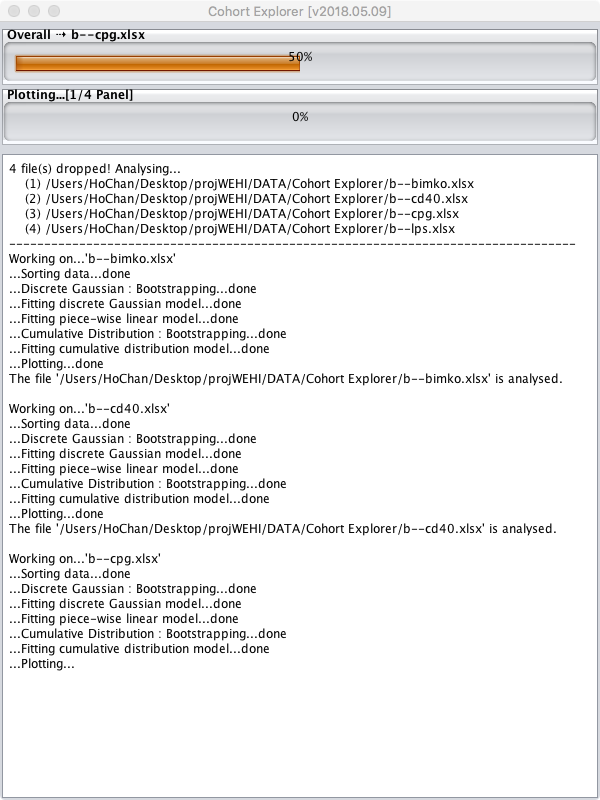
\includegraphics[scale=0.3]{./img/MainWindow-2_1.png}
        \centering
        \caption{Analysing state}
        \label{fig1b:analysing}
    \end{subfigure}
    \caption{Cohort Explorer Application}
\end{figure}
Multiple files can be dropped at once as shown in figure(\ref{fig1b:analysing}) but note that the program does not handle input files concurrently. The overall progress bar indicates percentage of completed files (out of all the input files) and the right arrow shows the current working file. The second progress bar displays the intermediate computation progress.

List of files and each computation steps are printed to the main screen in order to provide feedbacks and keep track of operations to the user. Should the program encounters any errors (e.g. unexpected excel format), it will terminate the analysis and reported back to user with clear error messages. Most common errors are raised due to data format so it is recommended to read Section \ref{sec:data_format} thoroughly and interrogate with provided example data before getting into the real one.

You will notice that the program automatically generates \textit{settings.txt} file if you run it for the first time. This is to set number of bootstrap iterations for calculating 95\% confidence intervals on every parameter estimations. More iteration number would contribute better parameter range, but it does not generally improve overall accuracy of the estimation. Keep in mind that higher iterations could result in expensive computation time, so adjust it for a good compromise between adequate report of confidence interval and speed.

%----------------------------------------------------------------------------------------
%	SECTION 1.2 : Output routines
%----------------------------------------------------------------------------------------
\subsection{Outputs}
There are three main output routines when analysis is done; (i) A secondary interactive window (figure \ref{fig:outputwindow}) to collect and display all the plots, (ii) one excel file that contain data points used for plotting as well as estimated parameters, (iii) individual plots in SVG and collected plots in PNG formats.

\begin{figure}[h]
    \centering
    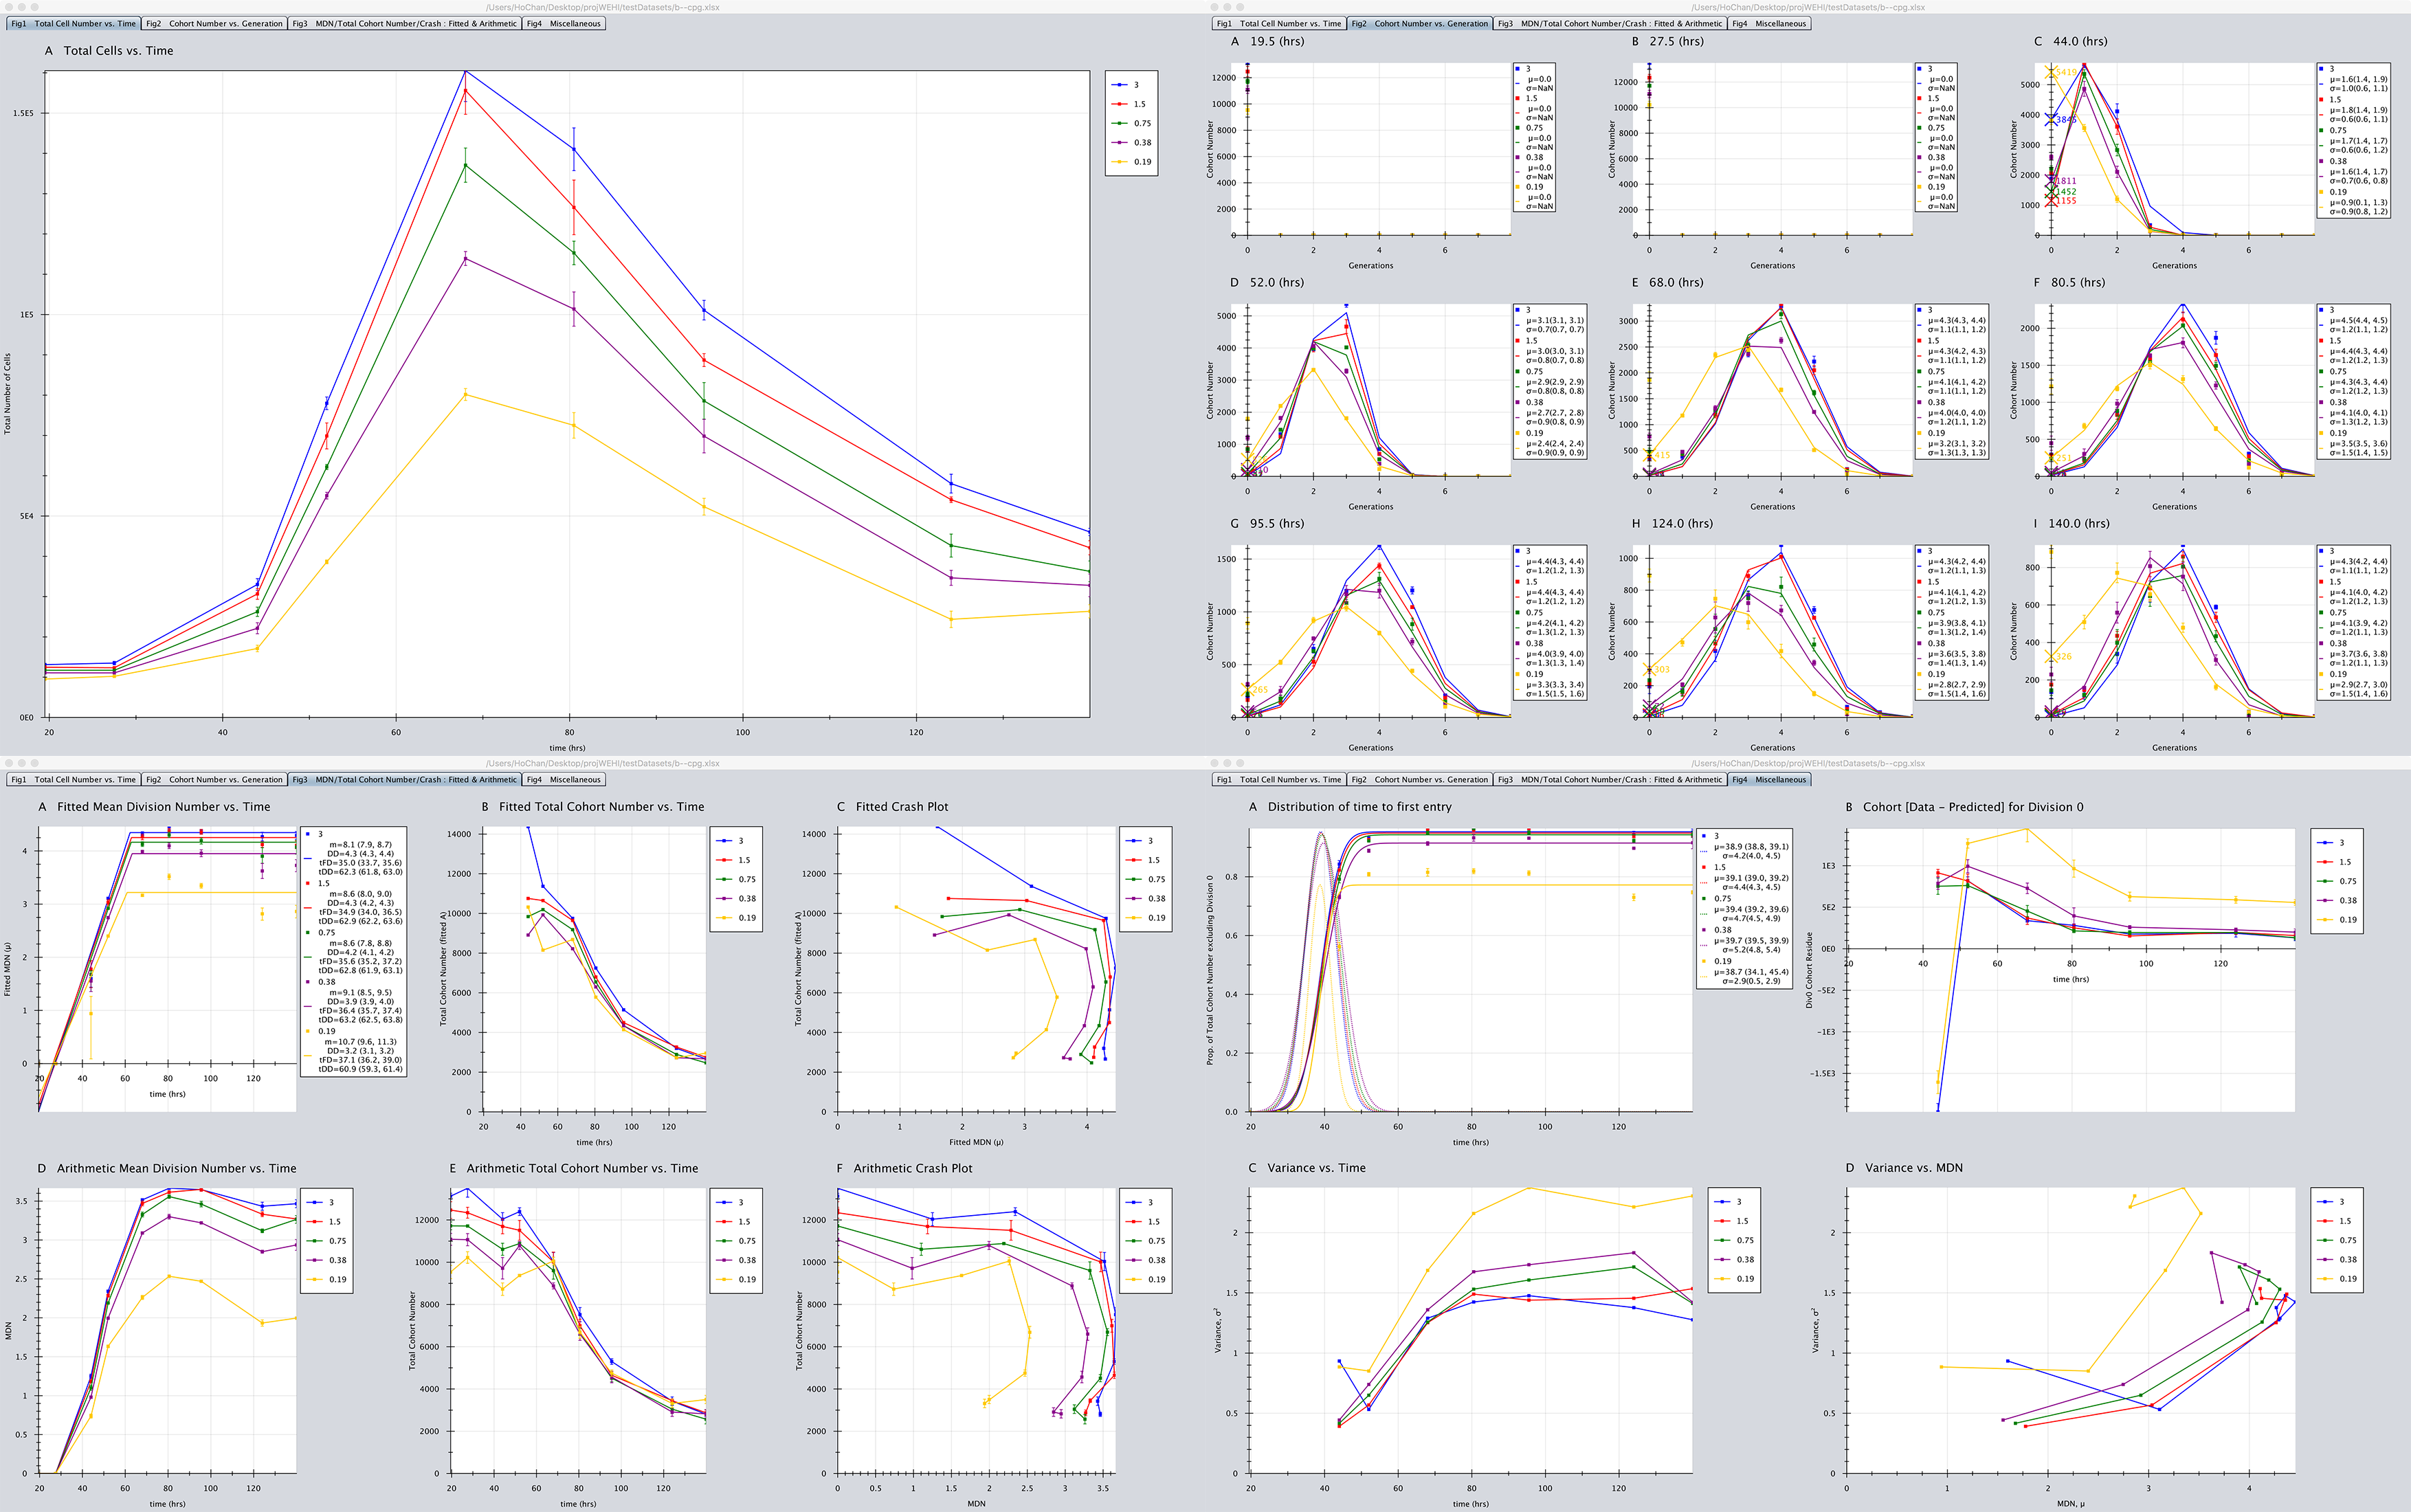
\includegraphics[scale=0.53]{./img/outputWindow.png}
    \caption{Interactive secondary window from example excel file ``b--cpg.xlsx"}
    \label{fig:outputwindow}
\end{figure}

All output files can be found on newly created directory named after input data file. Meta information such as time stamps, version of the program, and settings are printed in \textit{info.txt} for future reference. Note that output directory will not be overwritten should you run the program with same input file.

Figure numbers represent tab number in the interactive panel, and subfigures are labelled alphabetically (left to right, top to bottom in the panel) as a suffix to the figure number. Exported plots are named after their corresponding figure number and alphabets for consistency.
First tab of the panel shows evolution of the raw cell number counts for overview of the dynamics (square points: mean data $\pm$ S.E.M). If number of beads are present in your data it will calculate adjusted total cell number.

We then extract snapshots of the cell evolution, and plot them in the second tab in terms of cohort number as a function of generation. Each plot contains fitted discretised Gaussian curve with its estimated parameters displayed in respective legend (round bracket: 95\% confidence interval from bootstrap). Since generation 0 often contains noisy information (e.g. unstimulated/dead cells), we excluded this from best-fit and over plotted it with extrapolated generation 0 (marked as “X”) along with the actual data.

These results are then passed on to third tab to create summary plots of parameter evolution, and perform secondary piecewise fitting in order to draw more in depth cell kinematic parameters (tab 3 plot A). Notice that this tab is mainly for comparing two different mathematical approaches introduced in Overview section. The first row is a collection of fitted results from tab 2, and the second row is results from independent arithmetic cohort method.

Lastly, we fit cumulative distribution function (CDF) to ratio of sum of cohort number (excluding generation 0) to total cohort number (tab 4 plot A). This would effectively give us accumulative number of cells that are entering first generation. Therefore, it is possible to infer a distribution of average time to enter first division. Solid line is fitted CDF curve and dashed line is its complementary Gaussian distribution. Tab 4 plot B, C, and D are residue of extrapolated generation 0 and data, fitted variance as function of time, and variance against fitted mean division number respectively. These are information carried from tab 2, discrete Gaussian fitting results.

%----------------------------------------------------------------------------------------
%	SECTION 1.3 : Excel input data format
%----------------------------------------------------------------------------------------
\subsection{Excel data format}
\label{sec:data_format}
We have adopted a custom excel format (HL-SEP-2016) in order to match output style of FlowJo, a cell proliferation assay analysis software, so that you can simply copy and paste into a new or existing excel file. In this way, we can minimise amount of manual operations to prepare data, and potentially human errors. Column A comprises of experimental setup information whereas from column D to P are the main part of the cell count data. It is important to flag the excel file exactly as “HL-SEP-2016” in column B, row 1 because the program will look for this particular cell to confirm that input file is indeed in a correct format. This was implemented for future updates and backward compatibility should we introduce a new data format. An example data is shown in figure (\ref{fig:FormatHLSEP2016}).

\begin{figure}[h]
    \centering
    \begin{subfigure}[h]{1.0\linewidth}
        \centering
        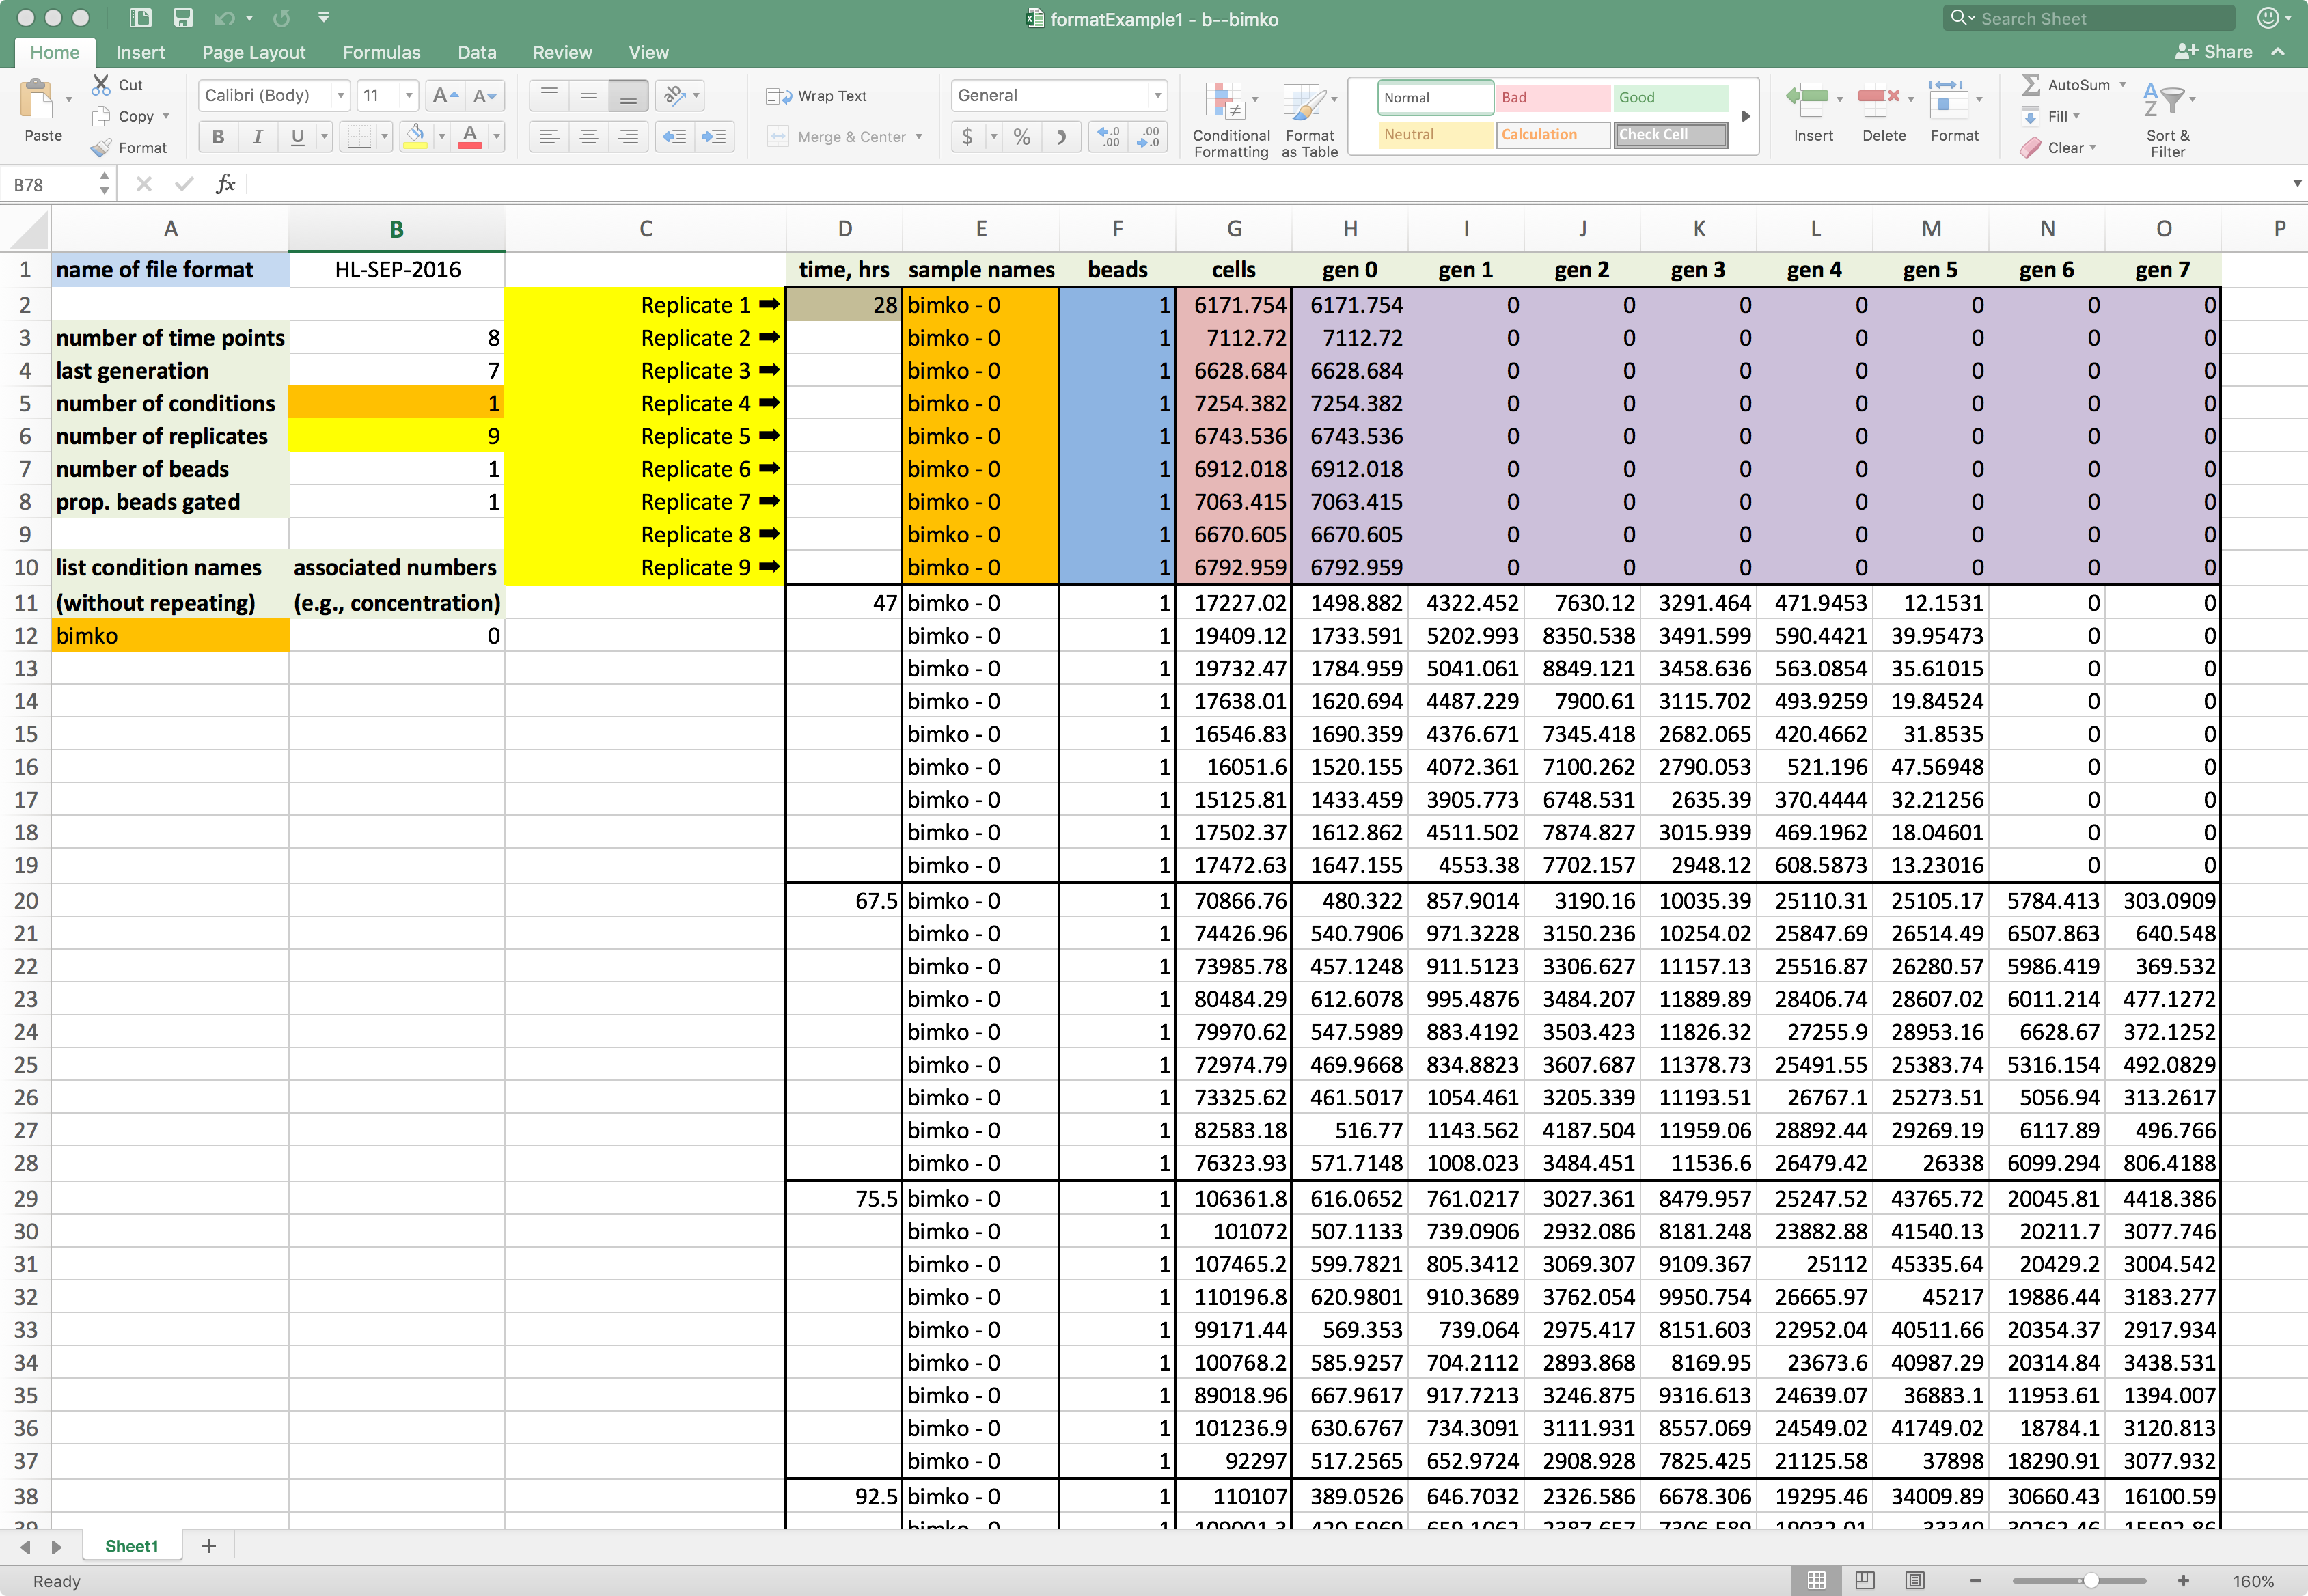
\includegraphics[scale=0.16]{./img/FormatHLSEP2016-1}
        \caption{One condition experiment with 9 replicates per condition}
        \label{fig:FormatHLSEP2016-1}
    \end{subfigure}
    \\
    \begin{subfigure}[h]{1.0\linewidth}
        \centering
        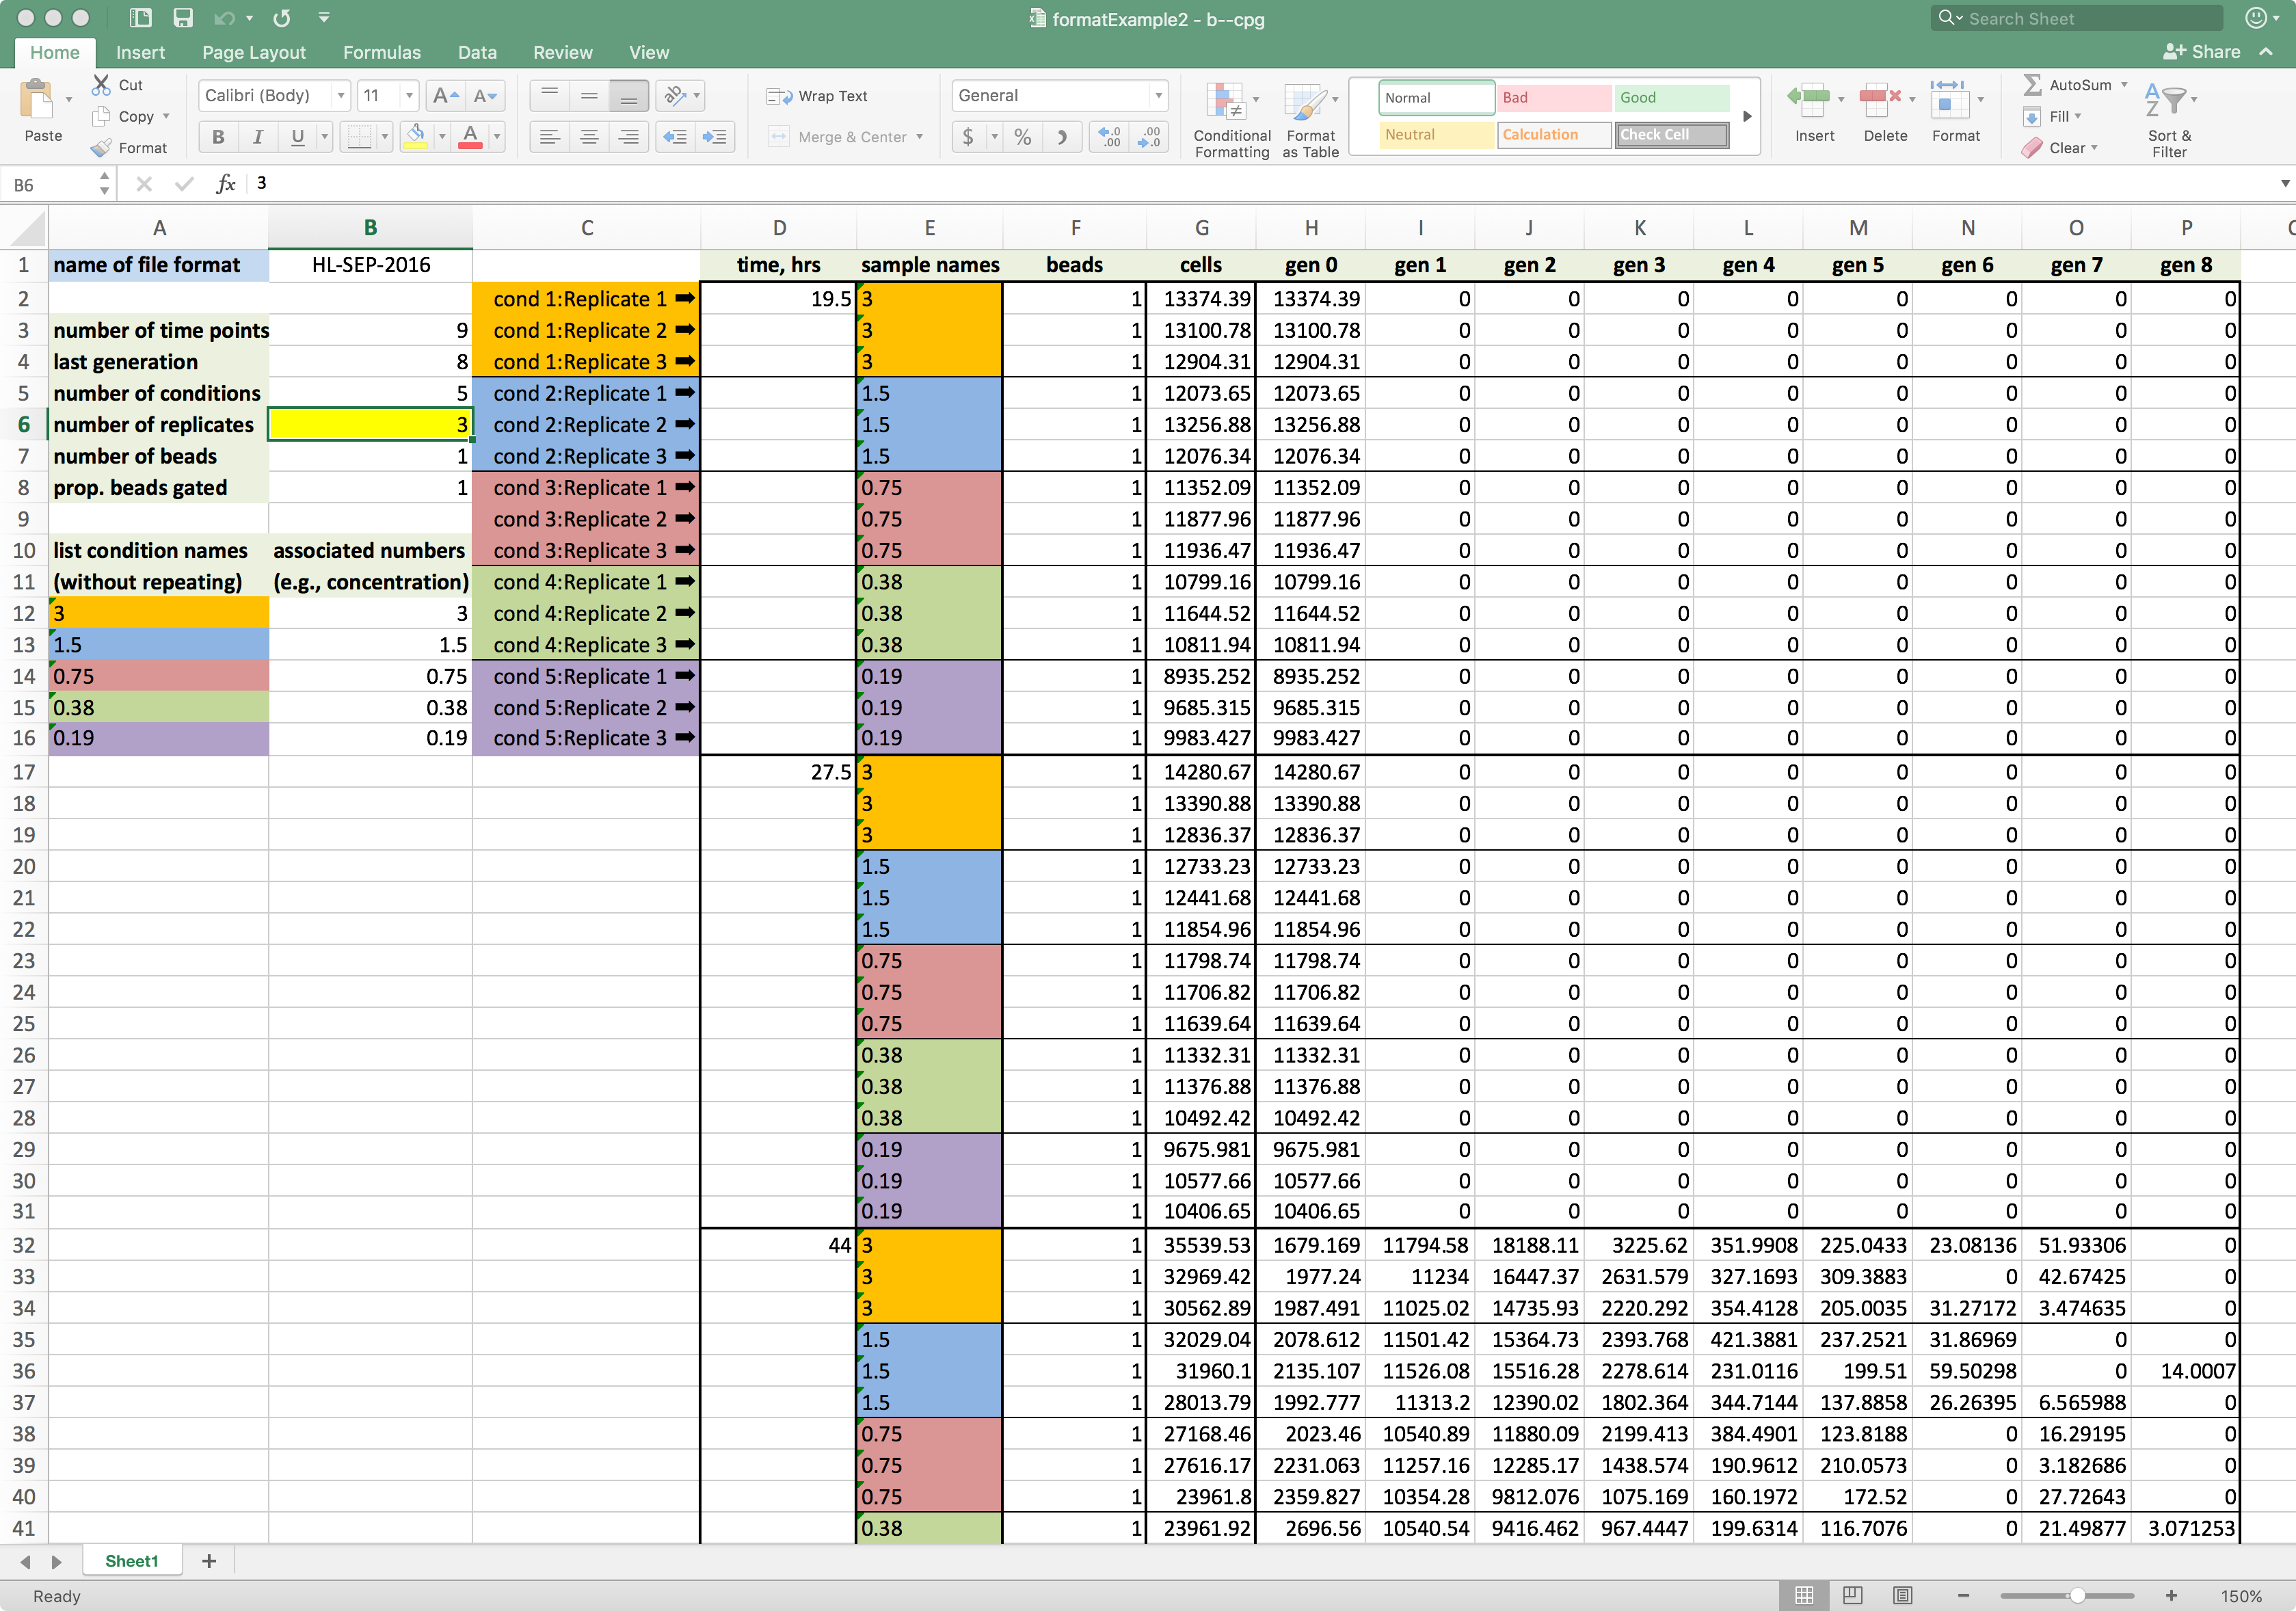
\includegraphics[scale=0.16]{./img/FormatHLSEP2016-2}
        \caption{Multiple conditions with 3 replicates per condition}
        \label{fig:FormatHLSEP2016-2}
    \end{subfigure}
    \caption{FormatHLSEP2016 Excel File}
    \label{fig:FormatHLSEP2016}
\end{figure}

Note the order of coloured blocks for differentiating various conditions. Each time point must have row number equal to number of conditions times number of replicates in an order that you specified in list condition names. If you have a missing replicate for particular condition, then leave the row blank to flag it as an empty replicate. The program will automatically adjust calculation (e.g. average cell number) during analysis.

%----------------------------------------------------------------------------------------
%	SECTION 1.4 : Flow Chart
%----------------------------------------------------------------------------------------
\clearpage
\subsection{Flow of Computation}
\begin{figure}[h]
    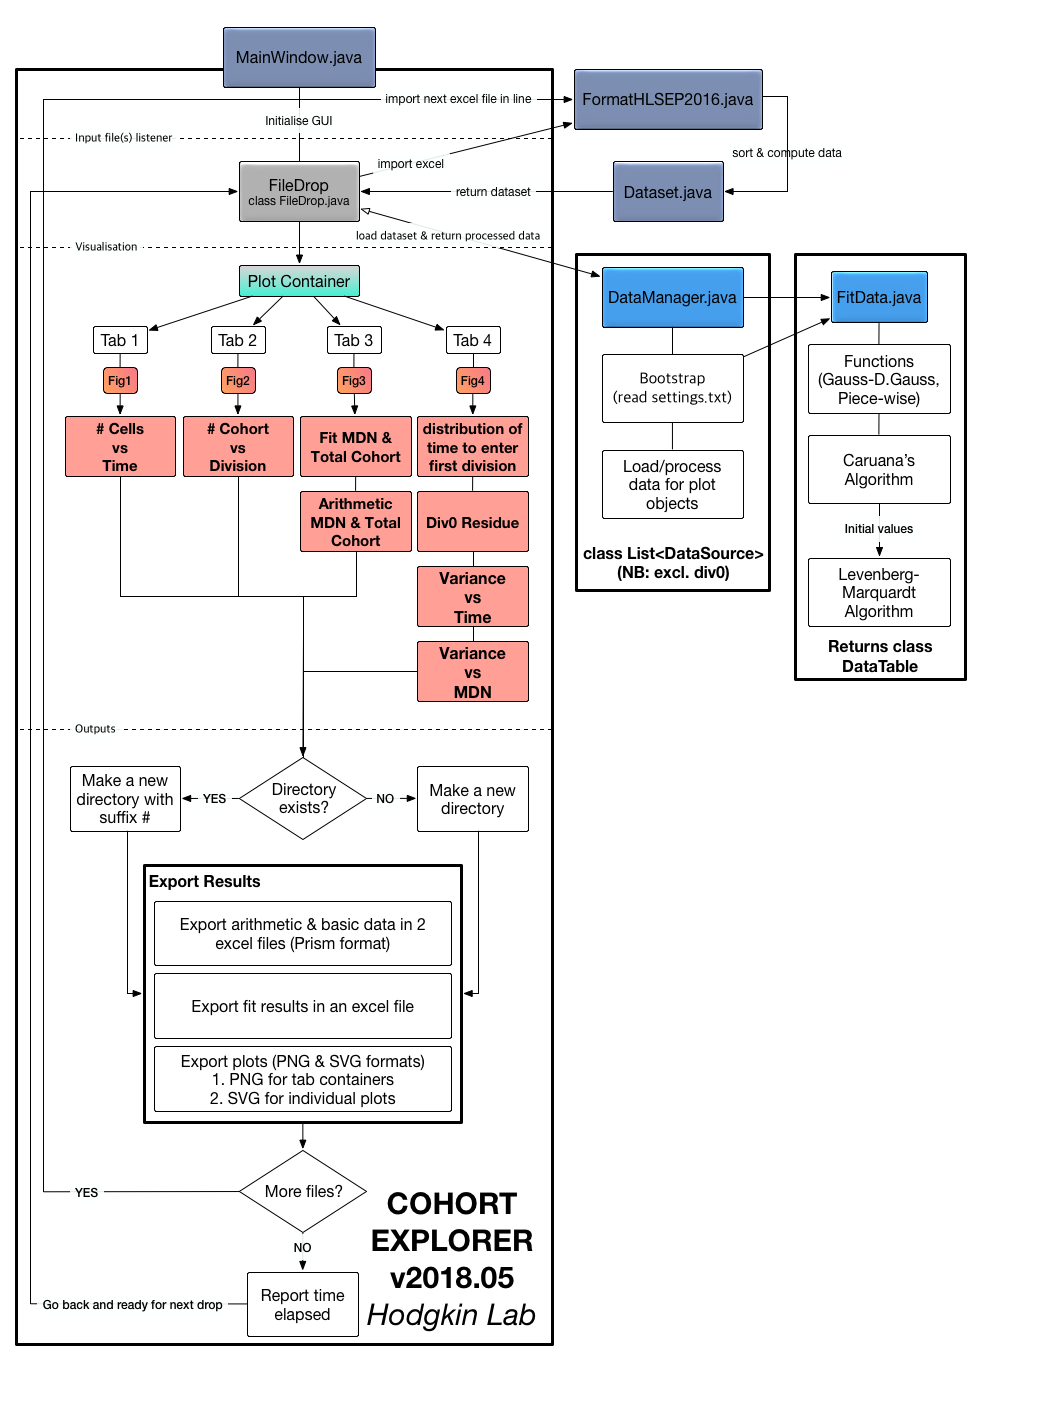
\includegraphics[scale=0.34]{./img/cohortFlow2.png}
    \centering
    \caption{Cohort Explorer - Flow Chart}
    \label{fig3:cohortFlow}
\end{figure}


%----------------------------------------------------------------------------------------
%	SECTION 2 : Fundamentals of cohort analysis
%----------------------------------------------------------------------------------------
\clearpage
\begin{homeworkProblem}[Preliminary Mathematics of Cohort Analysis]
Let $n(k,t)$ be number of cells at generation $k$ and at time $t$, then the cohort number is defined as
\begin{equation}
    c(k,t) = \frac{n(k,t)}{2^k},
    \label{eq:cohort_number}
\end{equation}
for a cell divides into two cells as it subsequently enters next generation. This allows us to construct a distribution of cohorts per time as a function of generation, cf. figure(\ref{fig:caruana_results}, \ref{fig:cohort_distribution}). Such distribution can be quantitatively analysed by two seemingly different methods, \textit{fitting} and \textit{arithmetic}, but ultimately shares same goals; computing mean division number (MDN), time to first division(tFD), division destiny(DD), and potentially many other biologically significant quantities of proliferation dynamics.

\end{homeworkProblem}
%----------------------------------------------------------------------------------------
%	SECTION 3 : Fitting method
%----------------------------------------------------------------------------------------
\begin{homeworkProblem}[Fitting Method]
\label{section:method_details}
% TODO: PUT SUB-SECTION "Least-squares Problem : Levenberg-Marquardt Algorithm"
\subsection{Least-squares Problem}
Given a set of data, $d_i = (x_i, y_i)$, and a model function, $f(x;\hat{\mathbf{p}})$, we can obtain parameters that minimise sum of square residues of the form,
\begin{equation}
    \operatornamewithlimits{argmin}\limits_{\hat{\mathbf{p}}} F(\hat{\mathbf{p}}) = \operatornamewithlimits{argmin}\limits_{\hat{\mathbf{p}}} ||\mathbf{r}(x_i;\hat{\mathbf{p}})||^2 = \sum_{i=1}^{N} [y_i - f(x_i;\hat{\mathbf{p}})]^2
\end{equation}
where $N$ is the number of data, $\hat{\mathbf{p}}$ is a parameter vector that its elements are minimisers of $r(x_i,\hat{\mathbf{p}})$. This is famous least-squares problem. Depending on linearity of a model function, different numerical technique is required. Simple linear functions involve solving a linear system of equations (e.g. $\mathbf{A}x = \mathbf{B}$) in which it is often solved by deploying linear algebra packages (or even analytically solved), whereas non-linear cases generally demand iterative procedure.

For our regression cohort analysis, we chose following list of non-linear functions for best fits,
\begin{enumerate}
    \item Discrete Gaussian function
    \item Piece-wise linear function with unknown breakpoints
    \item Cumulative distribution function
\end{enumerate}
All of which are non-linear with respect to corresponding parameters, thus, we implemented iterative numerical recipe called Levenberg-Marquardt(LM) algorithm \cite{Croeze, Griva, Madsen} with an aid of Caruana's method \cite{Guo, Pastuchova} as it is well accepted non-linear least-squares problem solver. It is frequently performed with constrains (with prior knowledge on experiments or mathematical anomalies) that bind parameter range but we did not implement any restriction to the algorithm.

As powerful as the algorithm can go, it also suffers from one major limitation. LM algorithm requires a set of initial guesses at the beginning of iteration, and convergence is known to be susceptible to the choice of starting values, especially for noisy data (relative to the model) and complex functions. We handle this problem by implementing a systematic procedure to generate educated guesses in order to minimise underfitting and adapt to input data as much as possible.

%----------------------------------------------------------------------------------------
%	SECTION 3.2 : Caruana's algorithm
%----------------------------------------------------------------------------------------
\subsection{Caruana's Algorithm}
\begin{figure}[t]
    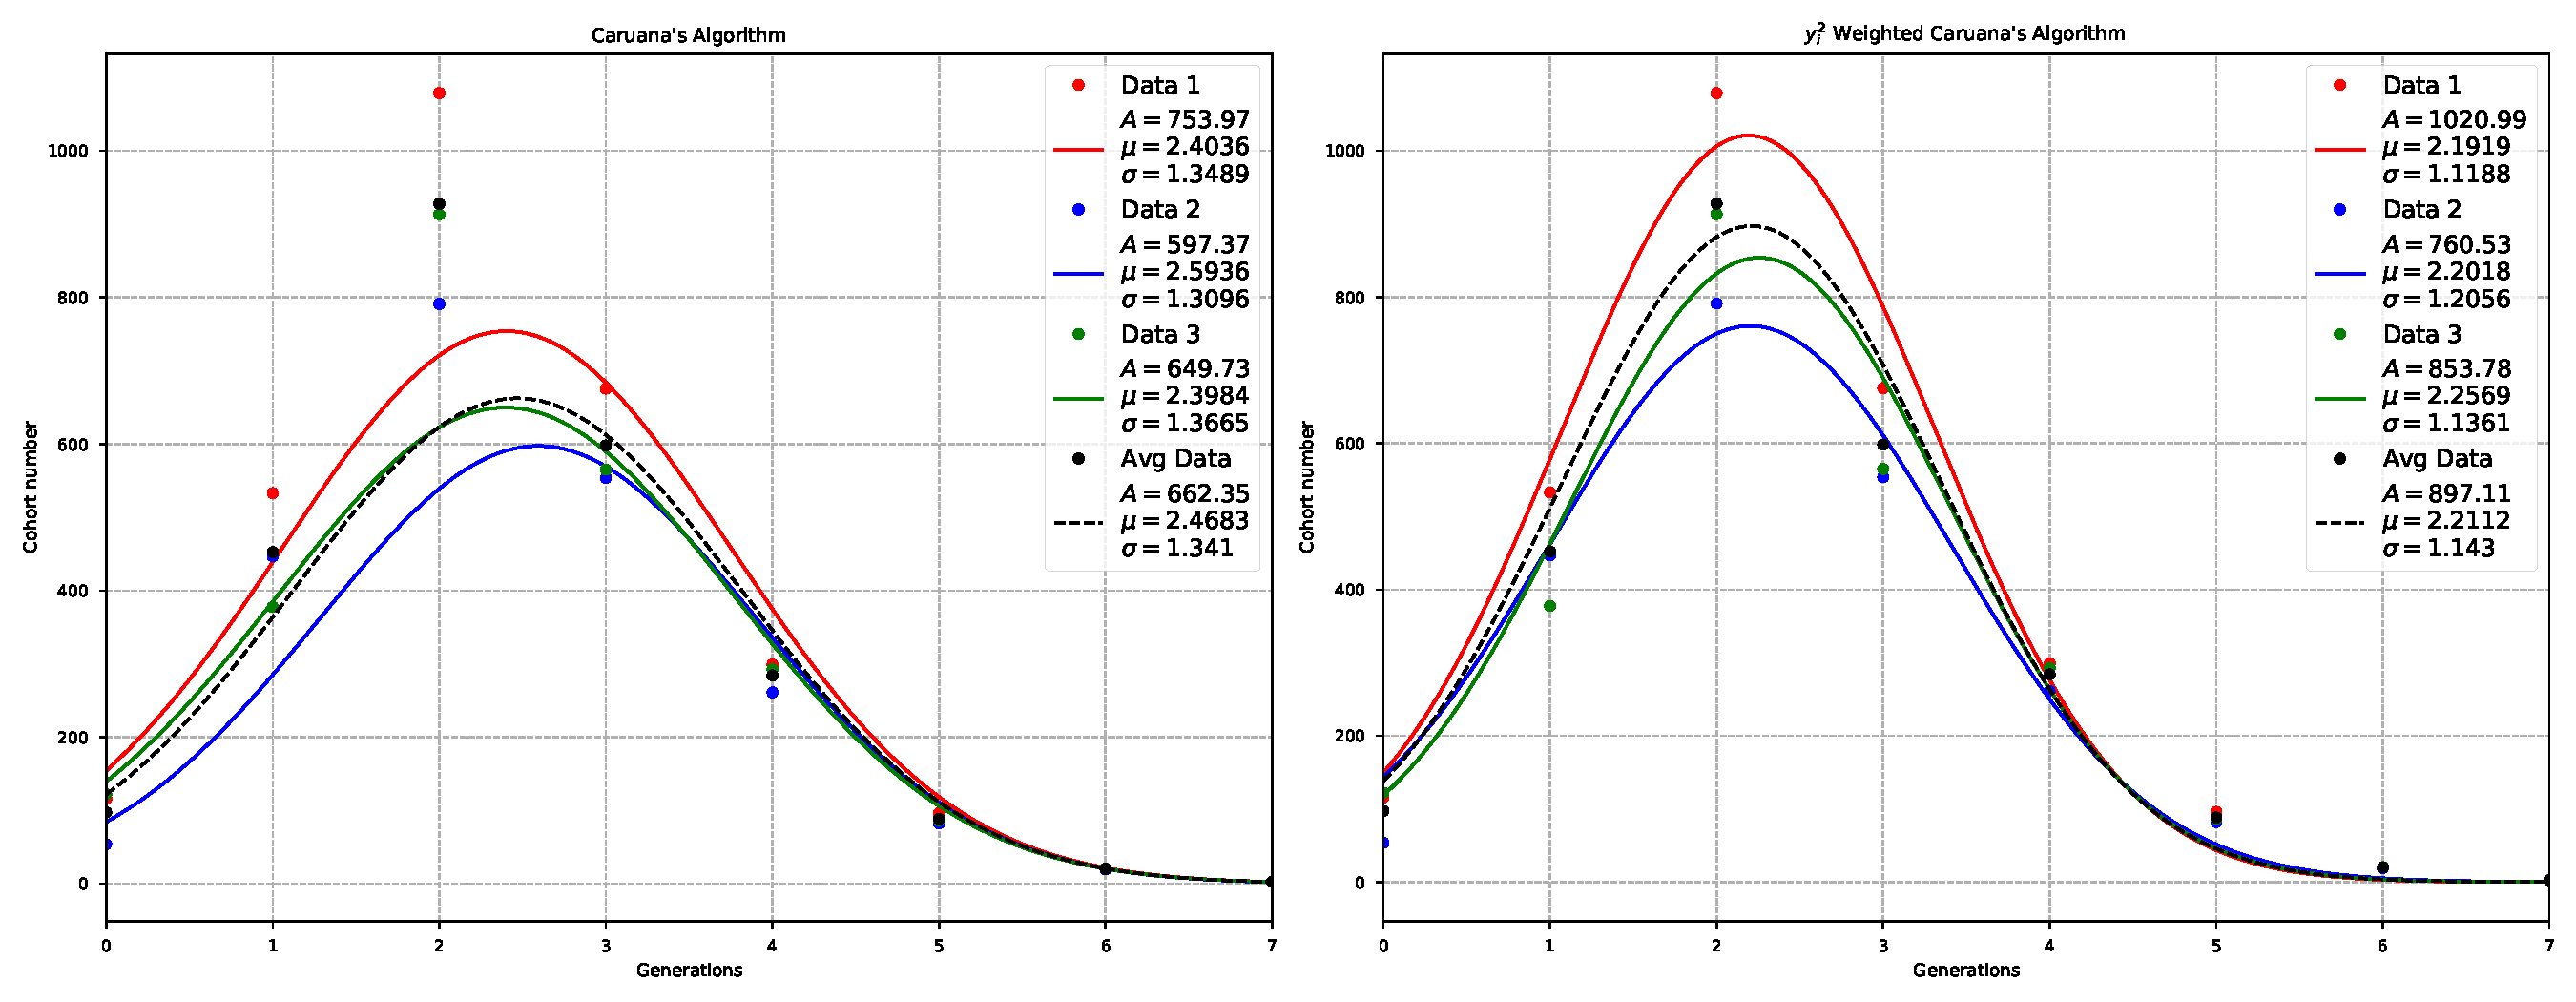
\includegraphics[scale=0.35]{./img/caruanaFit.pdf}
    \caption{\textbf{Example results of Caruana's algorithm.}}
    \centering
    \label{fig:caruana_results}
\end{figure}
The advantage of using Caruana's algorithm is that it does not require initial guesses.
The theory begins with linearising unnormalised Gaussian function, $f(x; \A, \MU, \SIGMA) \equiv y = \A e^{-(x-\MU)^2/2\SIGMA^2}$ by taking natural logarithm on both sides and expand to yield,
\begin{equation}
    \ln(y) = \ln(\A) - \frac{\MU^2}{2\SIGMA^2} + \frac{\MU}{\SIGMA^2}x - \frac{1}{2\SIGMA^2}x^2
\end{equation}
Let $\hat{a} =\ln(\A) -\MU^2 / 2\SIGMA^2$, $\hat{b} = \MU/\SIGMA^2$, and $\hat{c} = -1/2\SIGMA^2$, then equation is reduced to a second degree polynomial function,
\begin{equation}
    \ln(y) = \hat{a} + \hat{b}x + \hat{c}x^2
\end{equation}
So our residue function to minimise is,
\begin{equation}
    r(x_i; \hat{a}, \hat{b}, \hat{c}) = \ln(y_i) - (\hat{a} + \hat{b}x_i + \hat{c}x_i^2)
\end{equation}
Taking derivatives of $r^2$ with respect to $\hat{a}$, $\hat{b}$, and $\hat{c}$, and letting resultant expressions to zero produce linear system of equations,
\begin{align}
    \begin{bmatrix}
        N & \sum x_i & \sum x_i^2 \\
        \sum x_i & \sum x_i^2 & \sum x_i^3 \\
        \sum x_i^2 & \sum x_i^3 & \sum x_i^4
    \end{bmatrix}
    \begin{bmatrix}
        \hat{a} \\
        \hat{b} \\
        \hat{c}
    \end{bmatrix}
    =
    \begin{bmatrix}
        \sum \ln(y_i) \\
        \sum x_i \ln(y_i) \\
        \sum x_i^2 \ln(y_i)
    \end{bmatrix}
\end{align}
where $\sum$ runs through $N$ number of observed data. We can weight this equation by $y_i^2$ to yield,
\begin{equation}
    \begin{bmatrix}
     \sum y_i^2 & \sum x_iy_i^2 & \sum x_i^2y_i^2 \\
     \sum x_i y_i^2 & \sum x_i^2y_i^2 & \sum x_i^3y_i^2 \\
     \sum x_i^2y_i^2 & \sum x_i^3y_i^2 & \sum x_i^4y_i^2
    \end{bmatrix}
    \begin{bmatrix}
     \hat{a} \\
     \hat{b} \\
     \hat{c}
    \end{bmatrix}
    =
    \begin{bmatrix}
     \sum y_i^2 \ln(y_i) \\
     \sum x_iy_i^2 \ln(y_i) \\
     \sum x_i^2y_i^2 \ln(y_i)
    \end{bmatrix}
    \label{eq:caruana}
\end{equation}
After solving equation (\ref{eq:caruana}), parameters $(\hat{a},\hat{b},\hat{c})$ are converted back to original Gaussian parameters,
\begin{equation}
    \A = \exp\left[\hat{a} - \frac{\hat{b}^2}{4\hat{c}} \right], \qquad
    \MU = -\frac{\hat{b}}{2\hat{c}}, \qquad
    \SIGMA = \sqrt{-\frac{1}{2\hat{c}}}
\end{equation}
Both unweighted and weighted Caruana fit results are shown in Figure (\ref{fig:caruana_results}). It is not ideal algorithm for datasets that are heavily deviated from Gaussian distribution as it propagates errors logarithmically should the errors exist. However, this method is computationally inexpensive, and it can provide reasonable initial starting points for more sophisticated fitting algorithm.

%----------------------------------------------------------------------------------------
%	SECTION 3.3 : Discrete Gaussian fitting
%----------------------------------------------------------------------------------------
\subsection{Discrete Gaussian Fitting}
\begin{figure}[t]
    % \hspace{-10em}
    \centering
    \begin{subfigure}[ht]{0.49\linewidth}
        \centering
        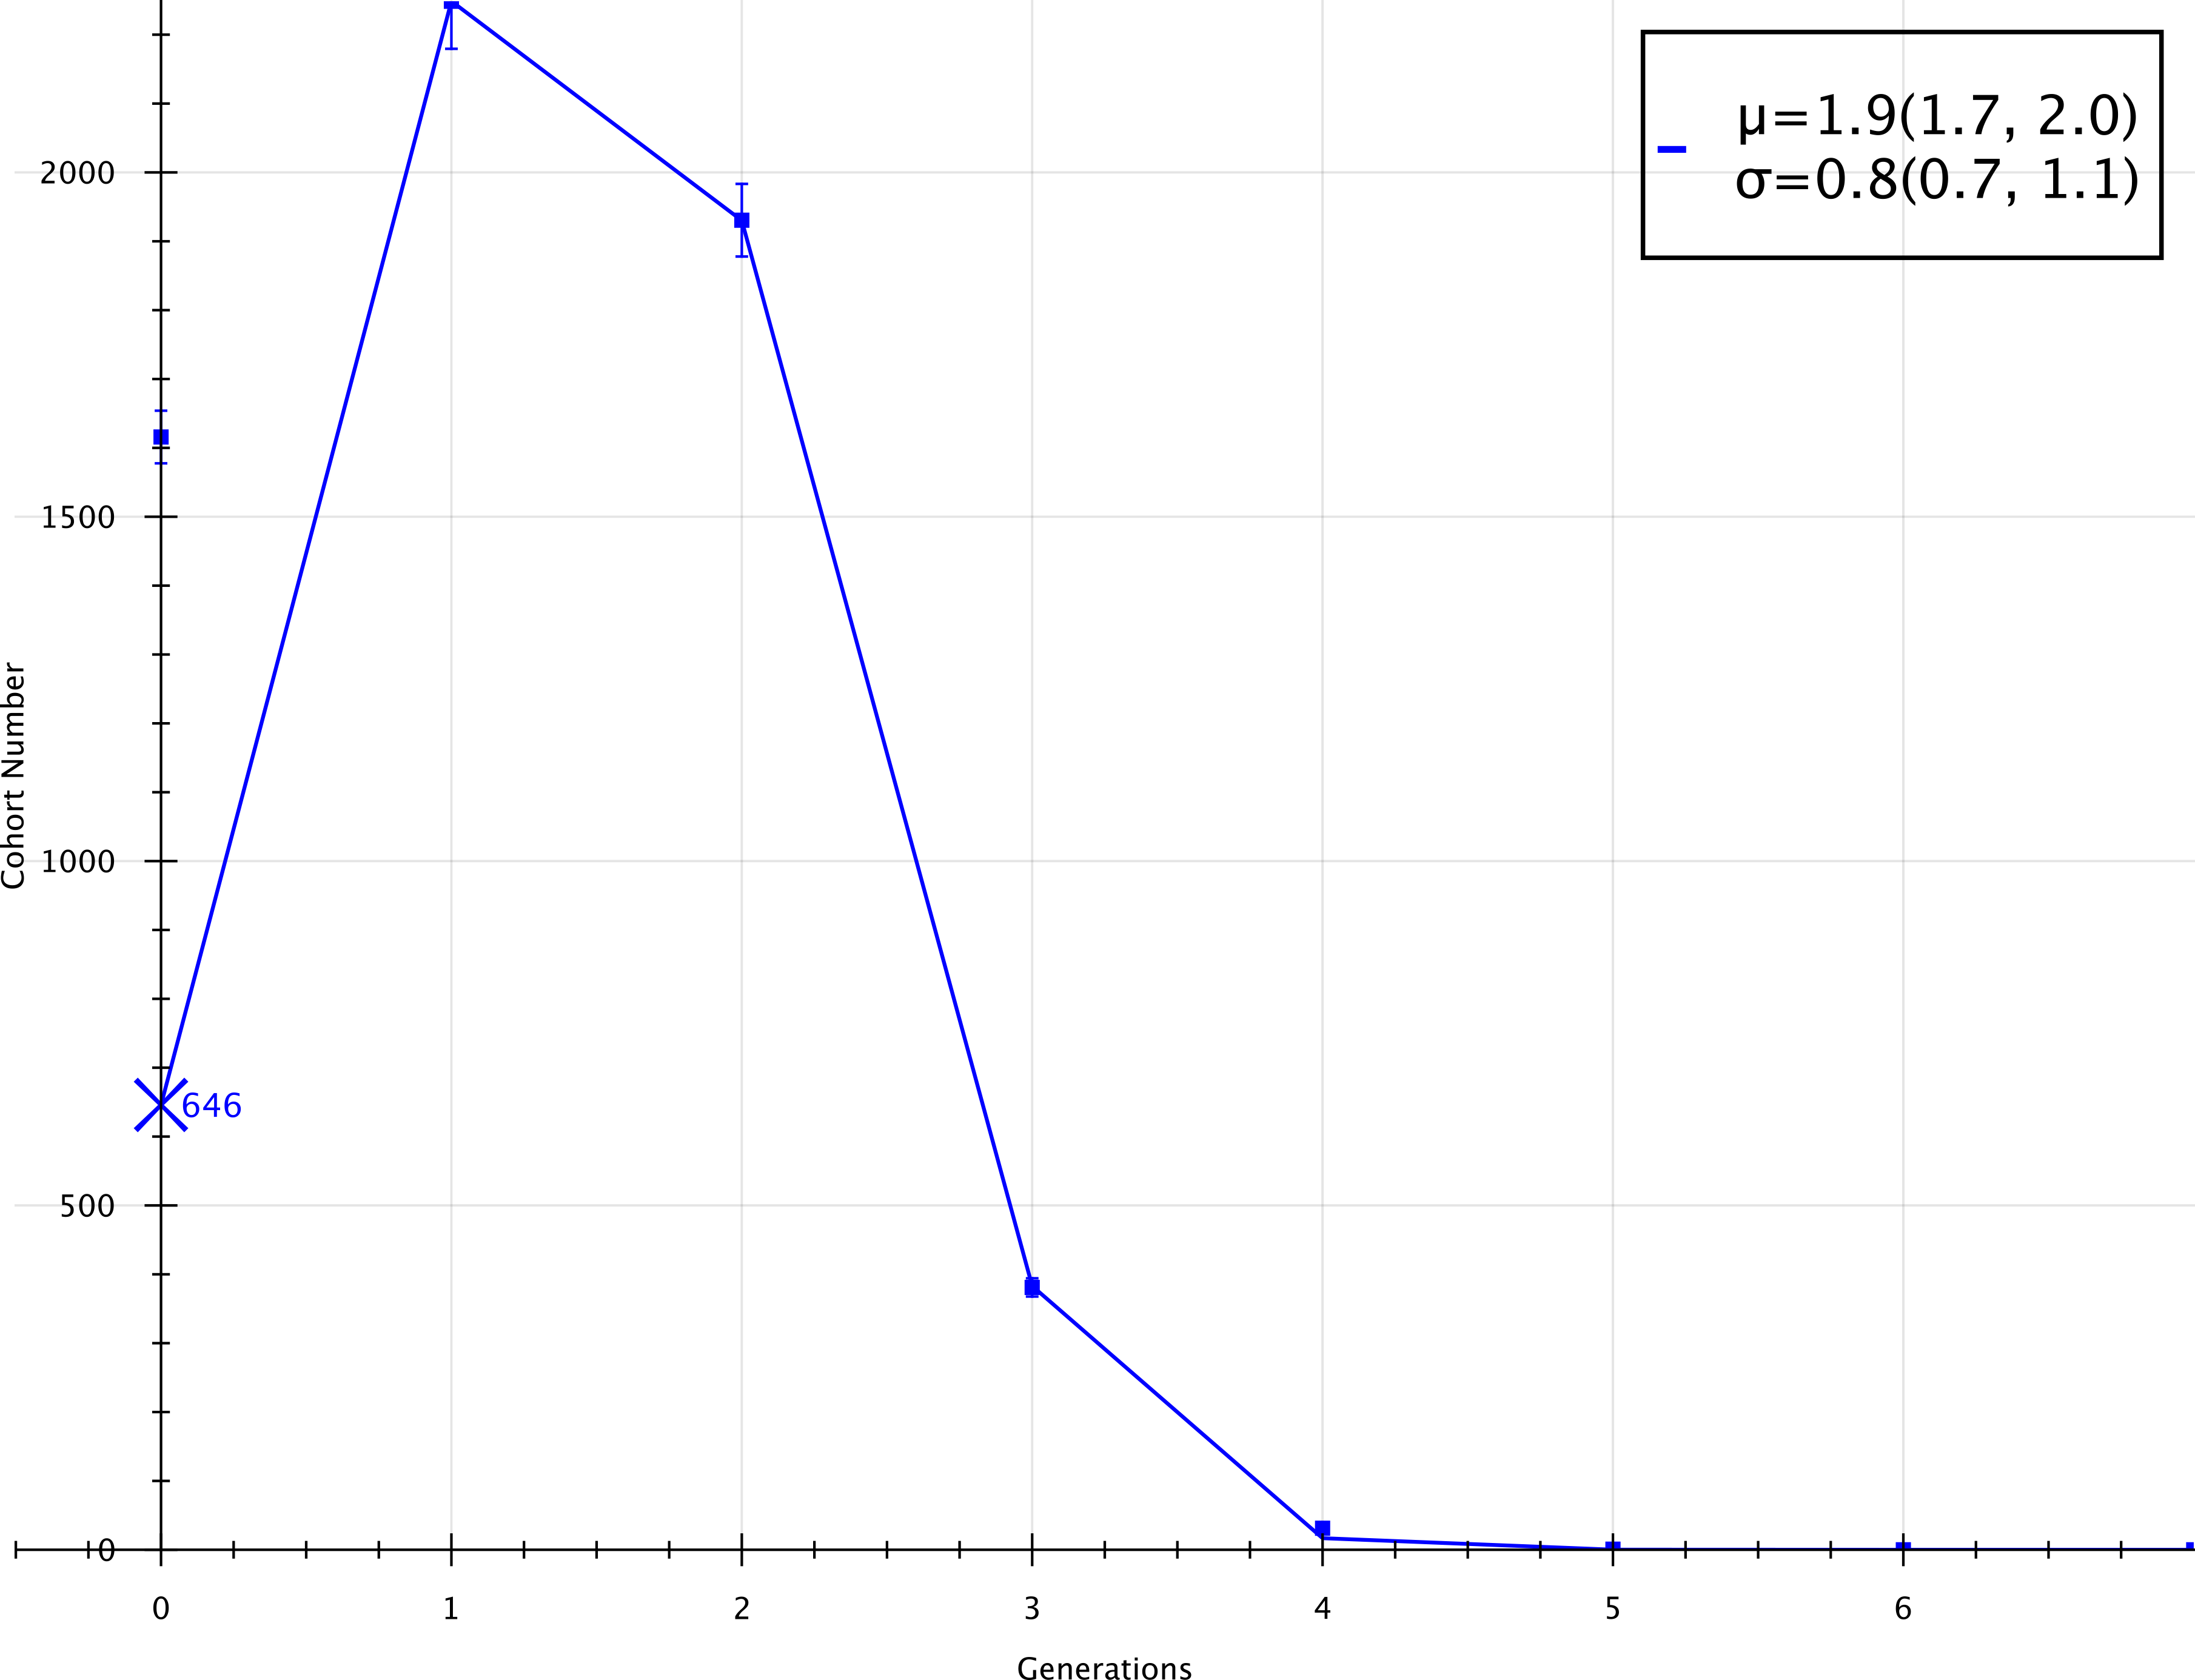
\includegraphics[scale=0.26]{./img/lmDGt0.png}
        \caption{Early time point: $\MU_{\mathrm{div}} = 1.9 \substack{+0.1 \\ -0.2}$  $\SIGMA_{\mathrm{div}} = 0.8 \substack{+0.3 \\ -0.1}$}
        \label{fig:DGt0}
    \end{subfigure}
    % \vspace{1em}
    \begin{subfigure}[ht]{0.49\linewidth}
        \centering
        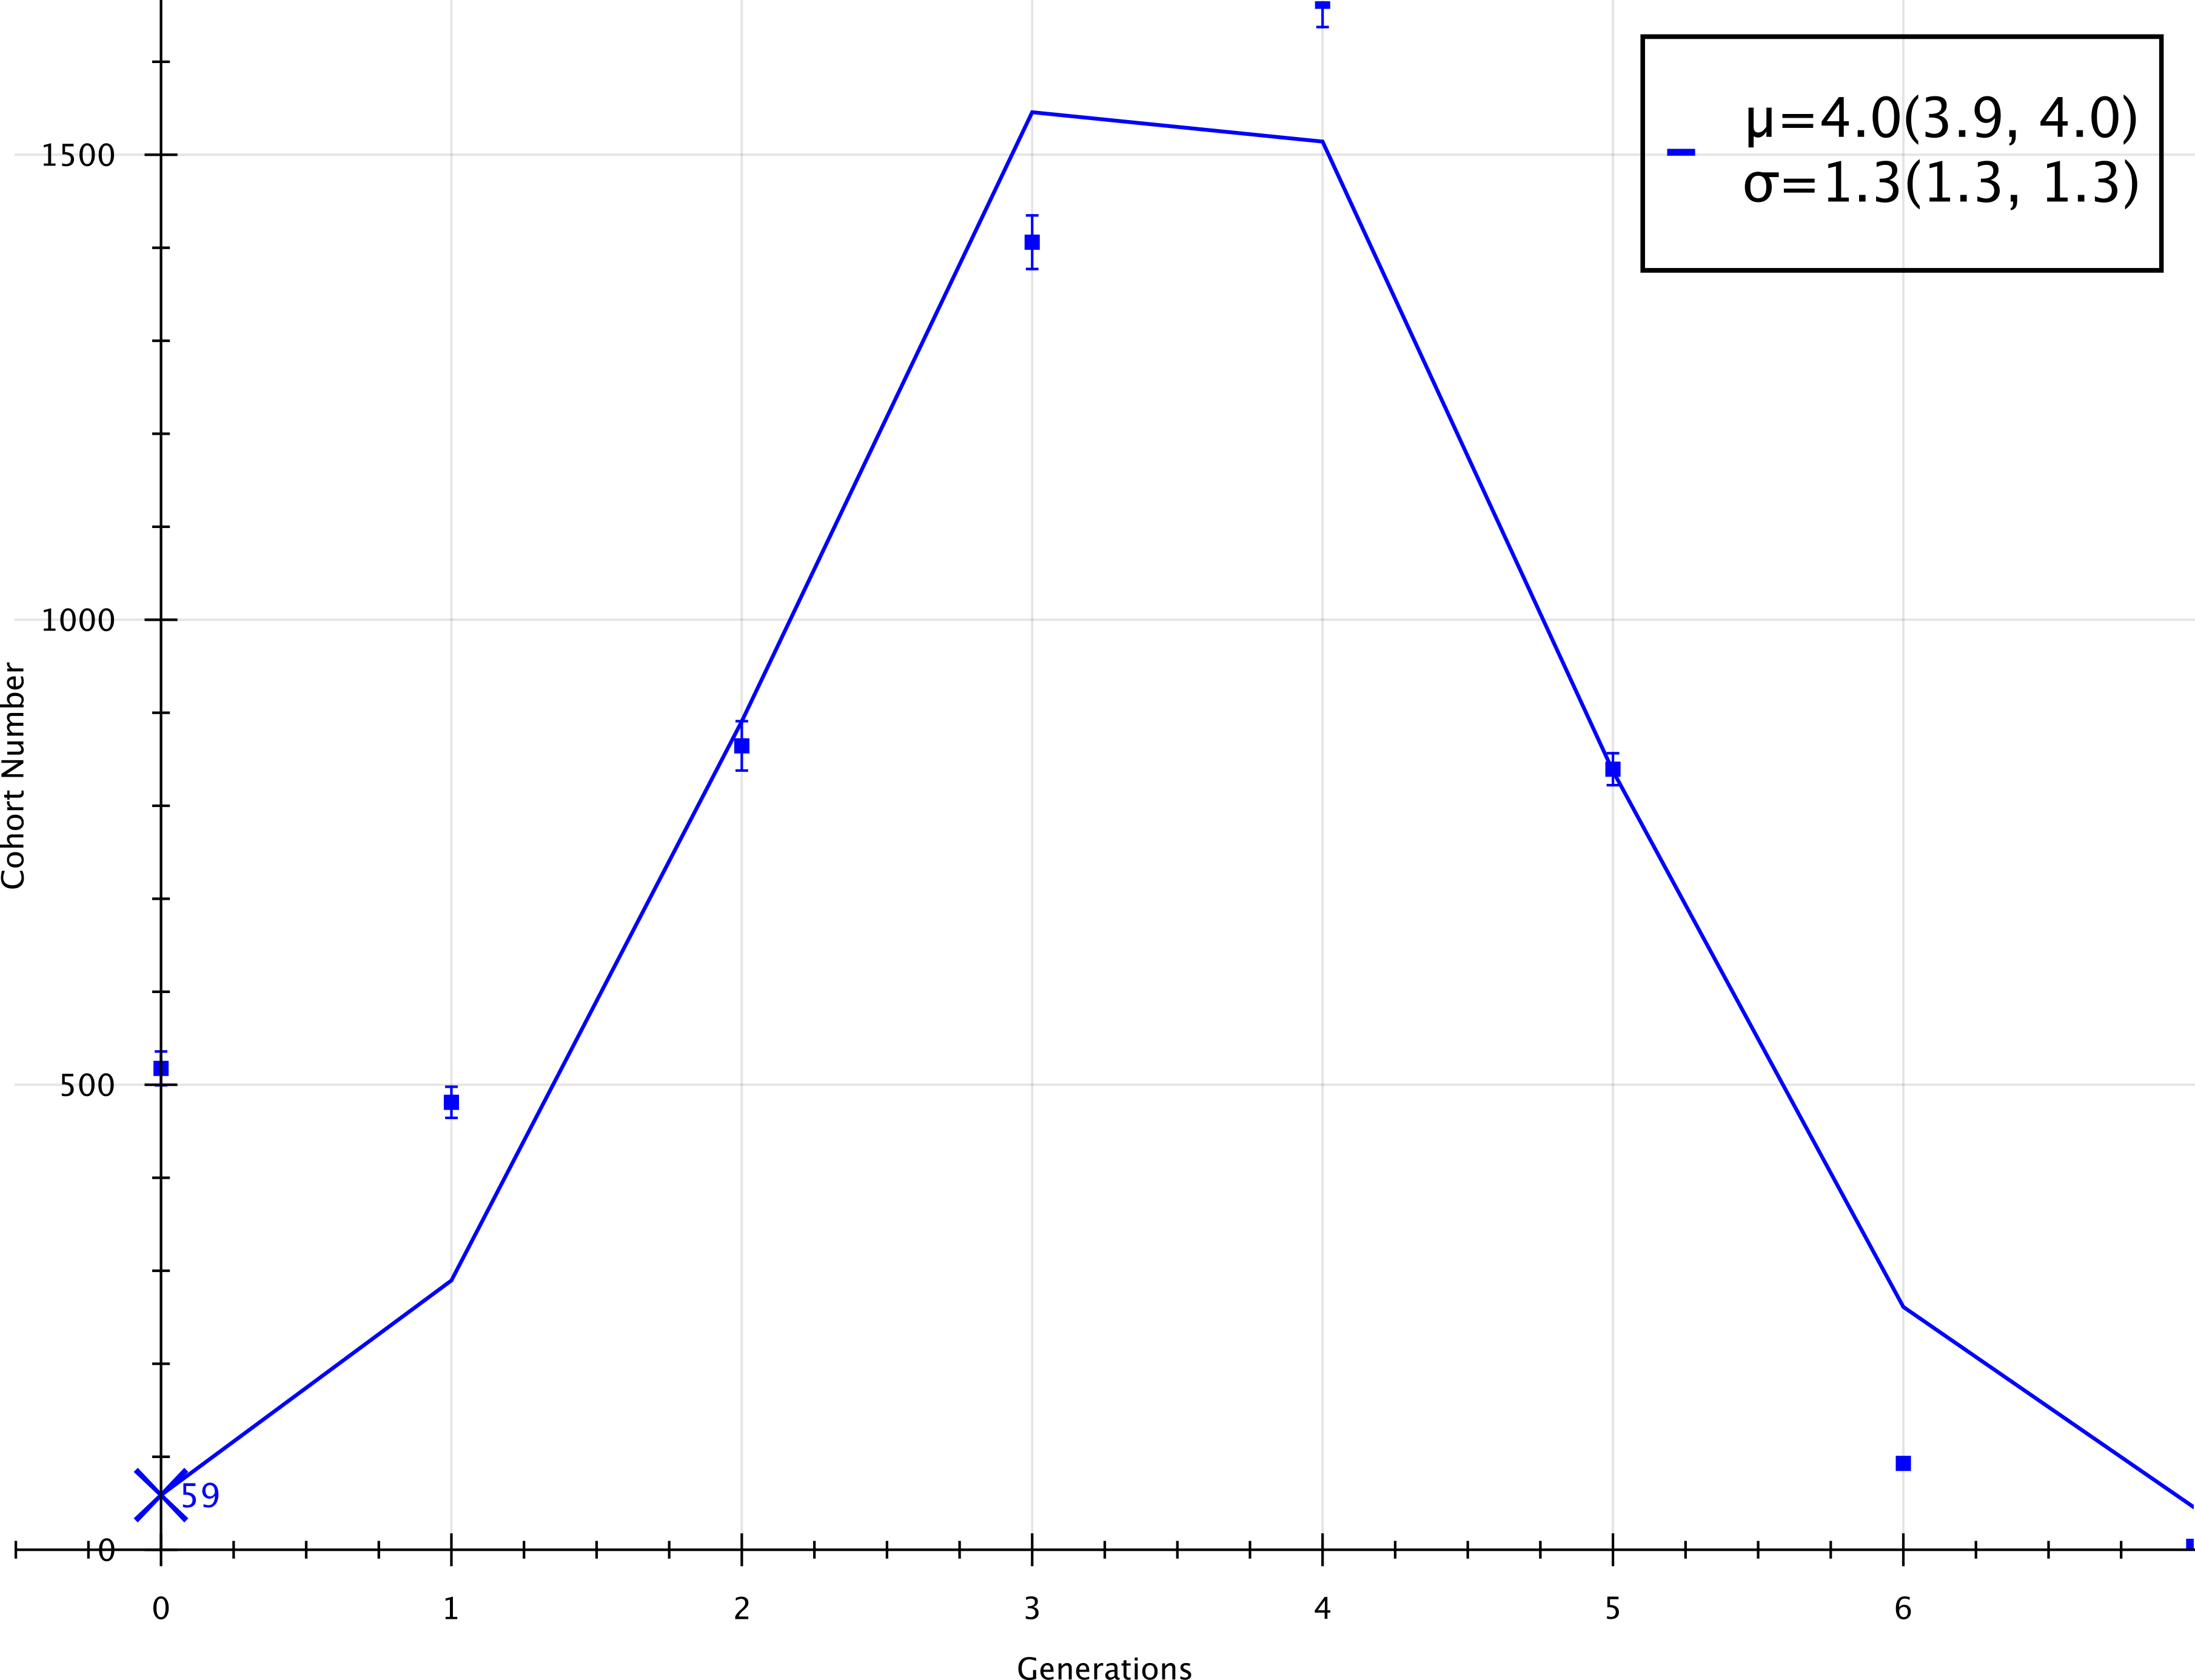
\includegraphics[scale=0.26]{./img/lmDGt1.png}
        \caption{Next time point: $\MU_{\mathrm{div}} = 4.0 \substack{+0.0 \\ -0.1}$  $\SIGMA_{\mathrm{div}} = 1.3 \substack{+0.0 \\ -0.0}$}
        \label{fig:DGt1}
    \end{subfigure}
    \caption{\textbf{Fitting equation (\ref{eq:discrete_gaussian_model}) to observed data collected at two different time points.} Solid Line - best fit, Data points = mean $\pm$ S.E.M. ``X" label is extrapolated generation 0 cohort number.}
    \label{fig:cohort_distribution}
\end{figure}
Recall unnormalised normal distribution,
\begin{equation}
    \N(k;\A', \MU_{\mathrm{div}}, \SIGMA_{\mathrm{div}}) = \A' \exp\left[-\frac{(k-\MU_{\mathrm{div}})^2}{2\SIGMA_{\mathrm{div}}^2}\right]
\end{equation}
where $k$ is generation, and $(\A', \MU{_\mathrm{div}}, \SIGMA_{\mathrm{div}})$ are the parameters to be estimated. It is reasonable model by itself for estimating distribution of cohorts, however, there is an experimental limitation we need to take into account. During the process of sorting data from flow cytometry, it is commonly practiced to bin cell counts by examining carboxyfluorescein succinimidyl ester (CFSE) profile. The profile generally shapes multimodal distribution, figure (\ref{fig:cfseProfile}), in which an operator semi-automatically gates cell counts per generation around the peaks. Inevitably, it is often hard to distinguish the exact boundaries of generations as cells do not discretely divide. Consider a cell in a mid way process to enter next generation (e.g. at generation 0.6). Because cells are continously distributed around the discrete generation number, essentially we are collapsing the datapoint as following:
\begin{align*}
    & \mathrm{gen}0 \leq \mathrm{data \ point} < \mathrm{gen}0.5 \ \rightarrow \ \mathrm{gen}0 \\
    & \mathrm{gen}0.5 \leq \mathrm{data \ point} < \mathrm{gen}1.5 \ \rightarrow \ \mathrm{gen}1 \\
    & \mathrm{gen}1.5 \leq \mathrm{data \ point} < \mathrm{gen}2.5 \ \rightarrow \ \mathrm{gen}2 \\
    & \qquad \qquad \qquad \qquad \vdots
\end{align*}
\begin{figure}
    \centering
    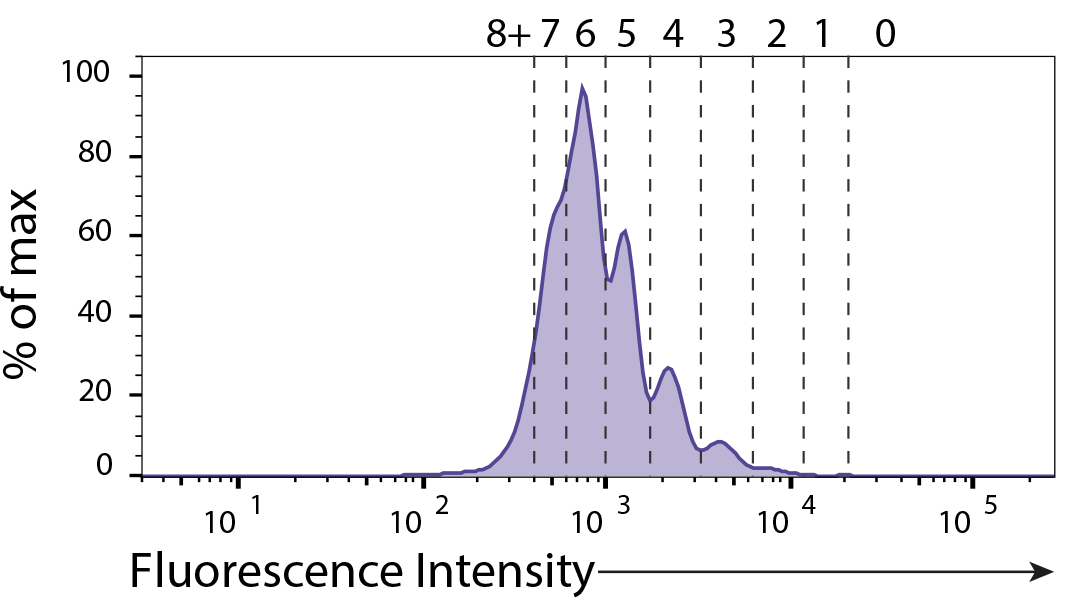
\includegraphics[scale=1.3]{./img/CTVgating.png}
    \caption{\textbf{CFSE profile using CellTrace Violet dye.} Cell division profile and gating of cell counts per generation shown as dash-lines. \textbf{CITE Tempany, Zhou, Bryant and Hodgkin}}
    \label{fig:cfseProfile}
\end{figure}
Evidently this would induce a selection bias toward the dataset, and propagates through remaining cohort analysis. This motivates us to apply mathmetical correction via discretising Gaussian model by integrating through consecutive generations.
\begin{equation}
    f(k;\A',\MU_{\mathrm{div}},\SIGMA_{\mathrm{div}}) = \int_{k}^{k+1} \N (k';\A',\MU_{\mathrm{div}},\SIGMA_{\mathrm{div}}) dk'
\end{equation}
which is equivalent to
\begin{equation}
    f(k;\A,\MU_{\mathrm{div}},\SIGMA_{\mathrm{div}}) = \left(\A\sqrt{2\pi\SIGMA_{\mathrm{div}}^2}\right)\frac{1}{2}\left[\erf\left(\frac{k+1-\MU_{\mathrm{div}}}{\SIGMA_{\mathrm{div}}\sqrt{2}}\right) - \erf\left(\frac{k-\MU_{\mathrm{div}}}{\SIGMA_{\mathrm{div}}\sqrt{2}}\right)\right]
    \label{eq:discrete_gaussian_model}
\end{equation}
where $\left(\A \sqrt{2\pi\SIGMA^2_{\mathrm{div}}}\right)$ is the total cohort number of particular dataset, and $\MU_{\mathrm{div}}$ is MDN that describes average generation of the cells.

Cell tracking technique can only detect cells up to certain generation (usually generation 7) before fluorescence dye that traces cell proliferation gets too diluted to be detected. This implies that ``last generation" is not a definitive termination of cell division, but rather experimental limitation on detecting (perhaps) existence of further generations. Hence, we implemented an additional correction to the data as following,
\begin{equation}
    c(k=\mathrm{last}, t) = \frac{\hat{n}(k,t)}{2^k} = \frac{1}{2^k}\sum_{i=k}^{\infty} 2^i \hat{c}(i)
\end{equation}
where $\hat{n}(k,t)$ is estimated total cell number beyond last generation, and $\hat{c}(i)$ is an extrapolated cohort number from the model, $f(k;\A,\MU_{\mathrm{div}},\SIGMA_{\mathrm{div}})$. It is obvious that the sum ideally needs to extend to the infinity but for computational purpose, we truncated it to 30 generation for a good approximation.

We repeatedly perform above corrections and fitting for all time points given in data, and the set of estimated $\MU_{\mathrm{div}}$ is then passed to construct a MDN time series plot, which then ultimately fitted to piece-wise linear function.

%----------------------------------------------------------------------------------------
%	SECTION 3.4 : Piece-wise fitting
%----------------------------------------------------------------------------------------
\subsection{Piece-wise Linear Fitting}
\begin{figure}[t]
    \centering
    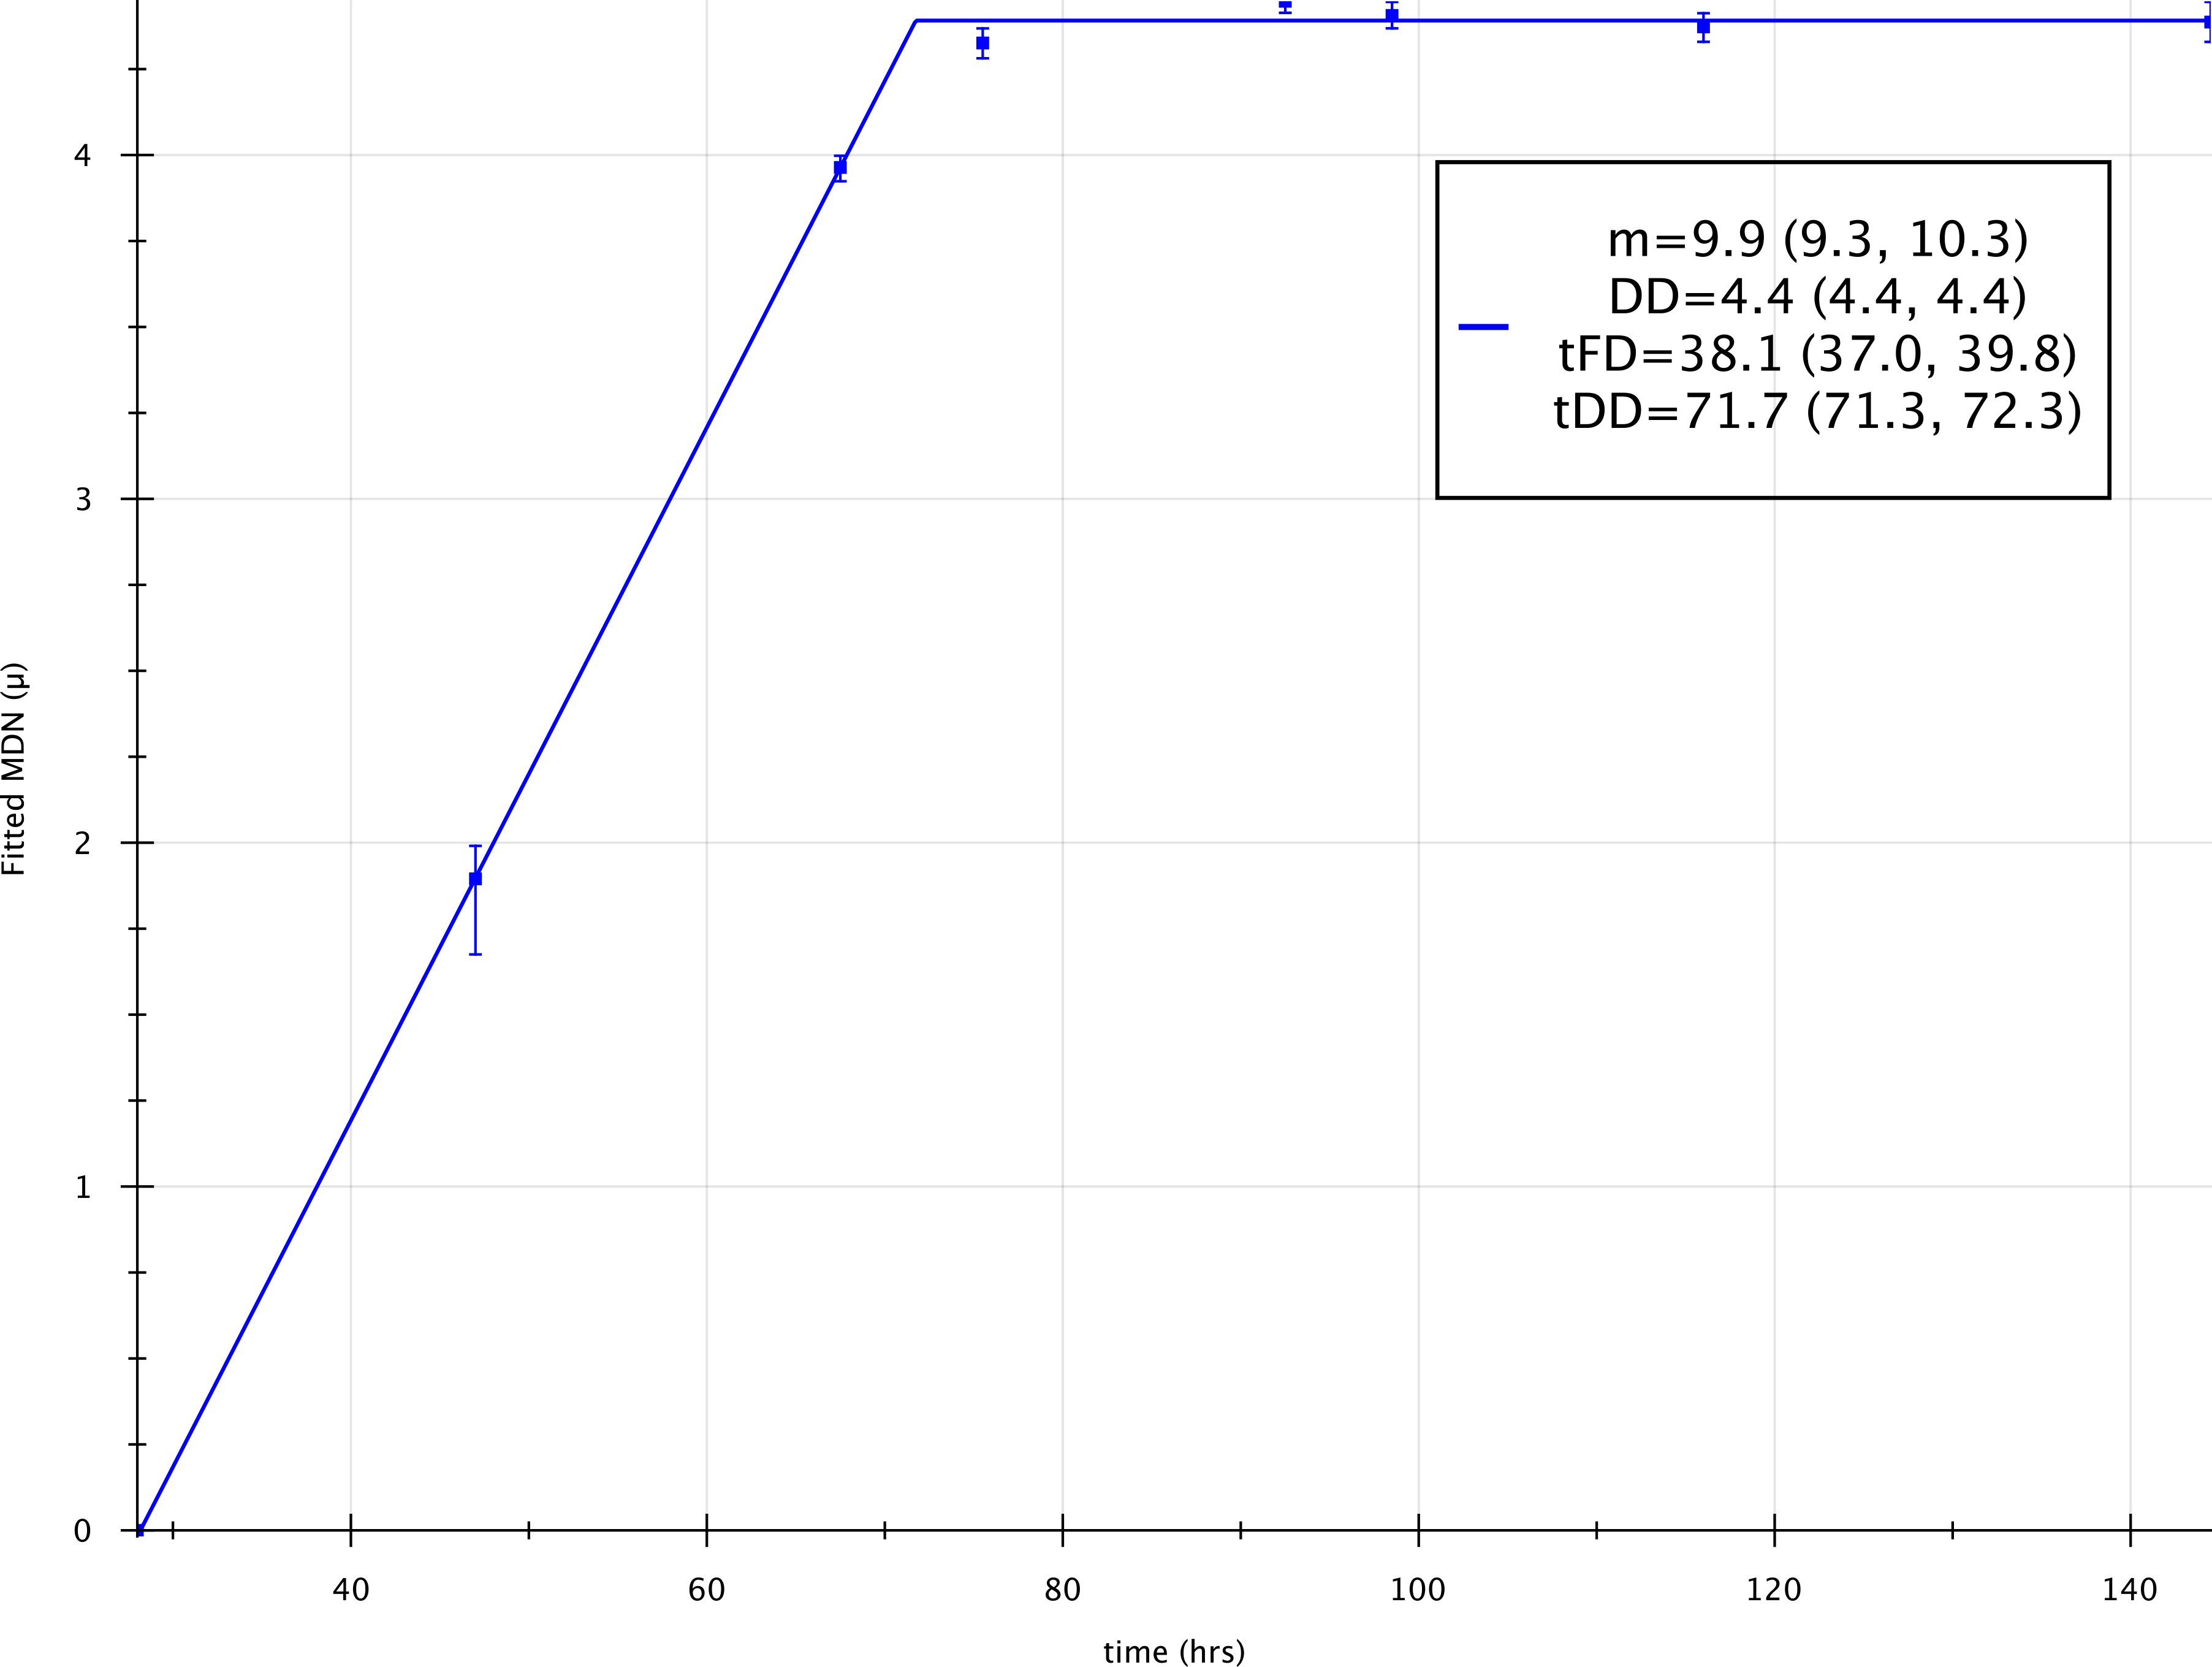
\includegraphics[scale=0.32]{./img/piecewise.png}
    \caption{\textbf{Piece-wise linear fitting with estimated set of $\mathbf{\MU_{\mathrm{div}}}$.} Error bars are 95\% confidence interval computed from bootstrapping. $m$ is time taken to enter subsequent division (k $\rightarrow$ k+1), $DD$ is generation that cell reaches its terminal division, $tFD$ is time when the cell enters first division, and $tDD$ is the break point that describes time when the cell enters division destiny.}
    \label{fig:piecewise}
\end{figure}
At first glance, one can expect that simple linear regression algorithm could be applied by splitting two regions and attach the estimated functions together. This can only be done if the break point is known prior to the fitting. However, it is generally an unknown quantity and is part of our main question to be answered.

We modified equation taken from Marsh et al. \cite{Marsh}, and run LM algorithm to explore parameter space of
\begin{equation}
    \label{eq:piecewise}
    g(t;\hat{a},\hat{b},\hat{bp}) = \hat{a} + \hat{b}\cdot t \cdot D_1 + \hat{b} \cdot \hat{bp} \cdot D_2
    \begin{cases}
        (D_1, D_2) = (1, 0), & \mathrm{if} \ t \leq bp \\
        (D_1, D_2) = (0, 1), & \mathrm{if} \ t > bp
    \end{cases}
\end{equation}
Note that equation (\ref{eq:piecewise}) is defined to be continuos at the break point but not necessarily differentiable. Once we have obtained ($\hat{a}, \hat{b}, \hat{bp}$) values, we can estimate time to enter subsequent division(m), time to first division(tFD), division destiny(DD), and time to division destiny(tDD):
\begin{equation}
    \mathrm{m} = \frac{1}{\hat{b}}, \qquad
    \mathrm{tFD} = \frac{1 - \hat{a}}{\hat{b}}, \qquad
    \mathrm{DD} = \hat{a} + \hat{b}\cdot \hat{bp}, \qquad
    \mathrm{tDD} = \hat{bp}
    \label{eq:piecewise_params}
\end{equation}
Since it is a secondary fitting procedure passed down from previous section, there could be hidden errors potentially propagated/amplified in the process. Consider following case: if majority of cells are not entering first division stage, then our cohort distribution is hardly look like a Gaussian distribution. This generally results in large 95\% confidence interval range, therefore, affects piece-wise fitting. In order to minimise this, we adjust LM algorithm to incoroperate errors by weighting each points with standard deivation computed by bootstrapping method.
\end{homeworkProblem}

%----------------------------------------------------------------------------------------
%	SECTION 4 : Arithmetic method details
%----------------------------------------------------------------------------------------
\begin{homeworkProblem}[Arithmetic Method]
In this section, we show alternative approach to compute previously derived quantities without any assumptions about the distribution. It is a simple arithmetic calculation in order to obtain statistical moments but not necessarily for further parameter estimation. Total cohort number is summation of equation (\ref{eq:cohort_number}) for all generation,
\begin{equation}
    S(t) = \sum_{k=0}^{\infty} c(k,t)
        \label{eq:total_cohort}
\end{equation}
This is equivalent to amplitude of the fitted discrete Gaussian function. Then we calculate average generation by summing weighted cohort number with respective generation number and divide the sum by total cohort number,
\begin{equation}
    h(t) = \sum_{k=0}^{\infty} \frac{k c(k,t)}{S(t)}
    \label{eq:MDN}
\end{equation}
Using equation (\ref{eq:MDN}), we can obtain similar plot to figure (\ref{fig:piecewise}). Notice that arithemtic and fitting methods produce different results even though they share same biological property. There are three critical reasons,
\begin{enumerate}
    \item Arithmetic method does not make correction (discretisation) to the dataset. This is a major factor that generally shifts MDN values.
    \item Dataset exhibits non-Gaussian distribution. In this particular case, estimated MDNs are unreliable, and it is shown by broad confidence interval (i.e. error bars).
    \item Fitting method can explore negative MDN region. It is a feature of unconstrained best-fit algorithm, which we take advantage of in order to investigate regime otherwise impossible to extrapolated by arithemtic method. This is debatable on how to interpret negative MDN estimations.
\end{enumerate}
It becomes a non-trivial problem to generalise and make realiable fitting algorithm for all possible datasets. As such, we provide outcomes from least assumed method side by side with fitting method so that you can choose a method that works best for your dataset.

%----------------------------------------------------------------------------------------
%	SECTION 4.1 : Cumulative distribution fitting
%---------------------------------------------------------------------------------------
\subsection{Cumulative Distribution Fitting}
\begin{figure}[t]
    \centering
    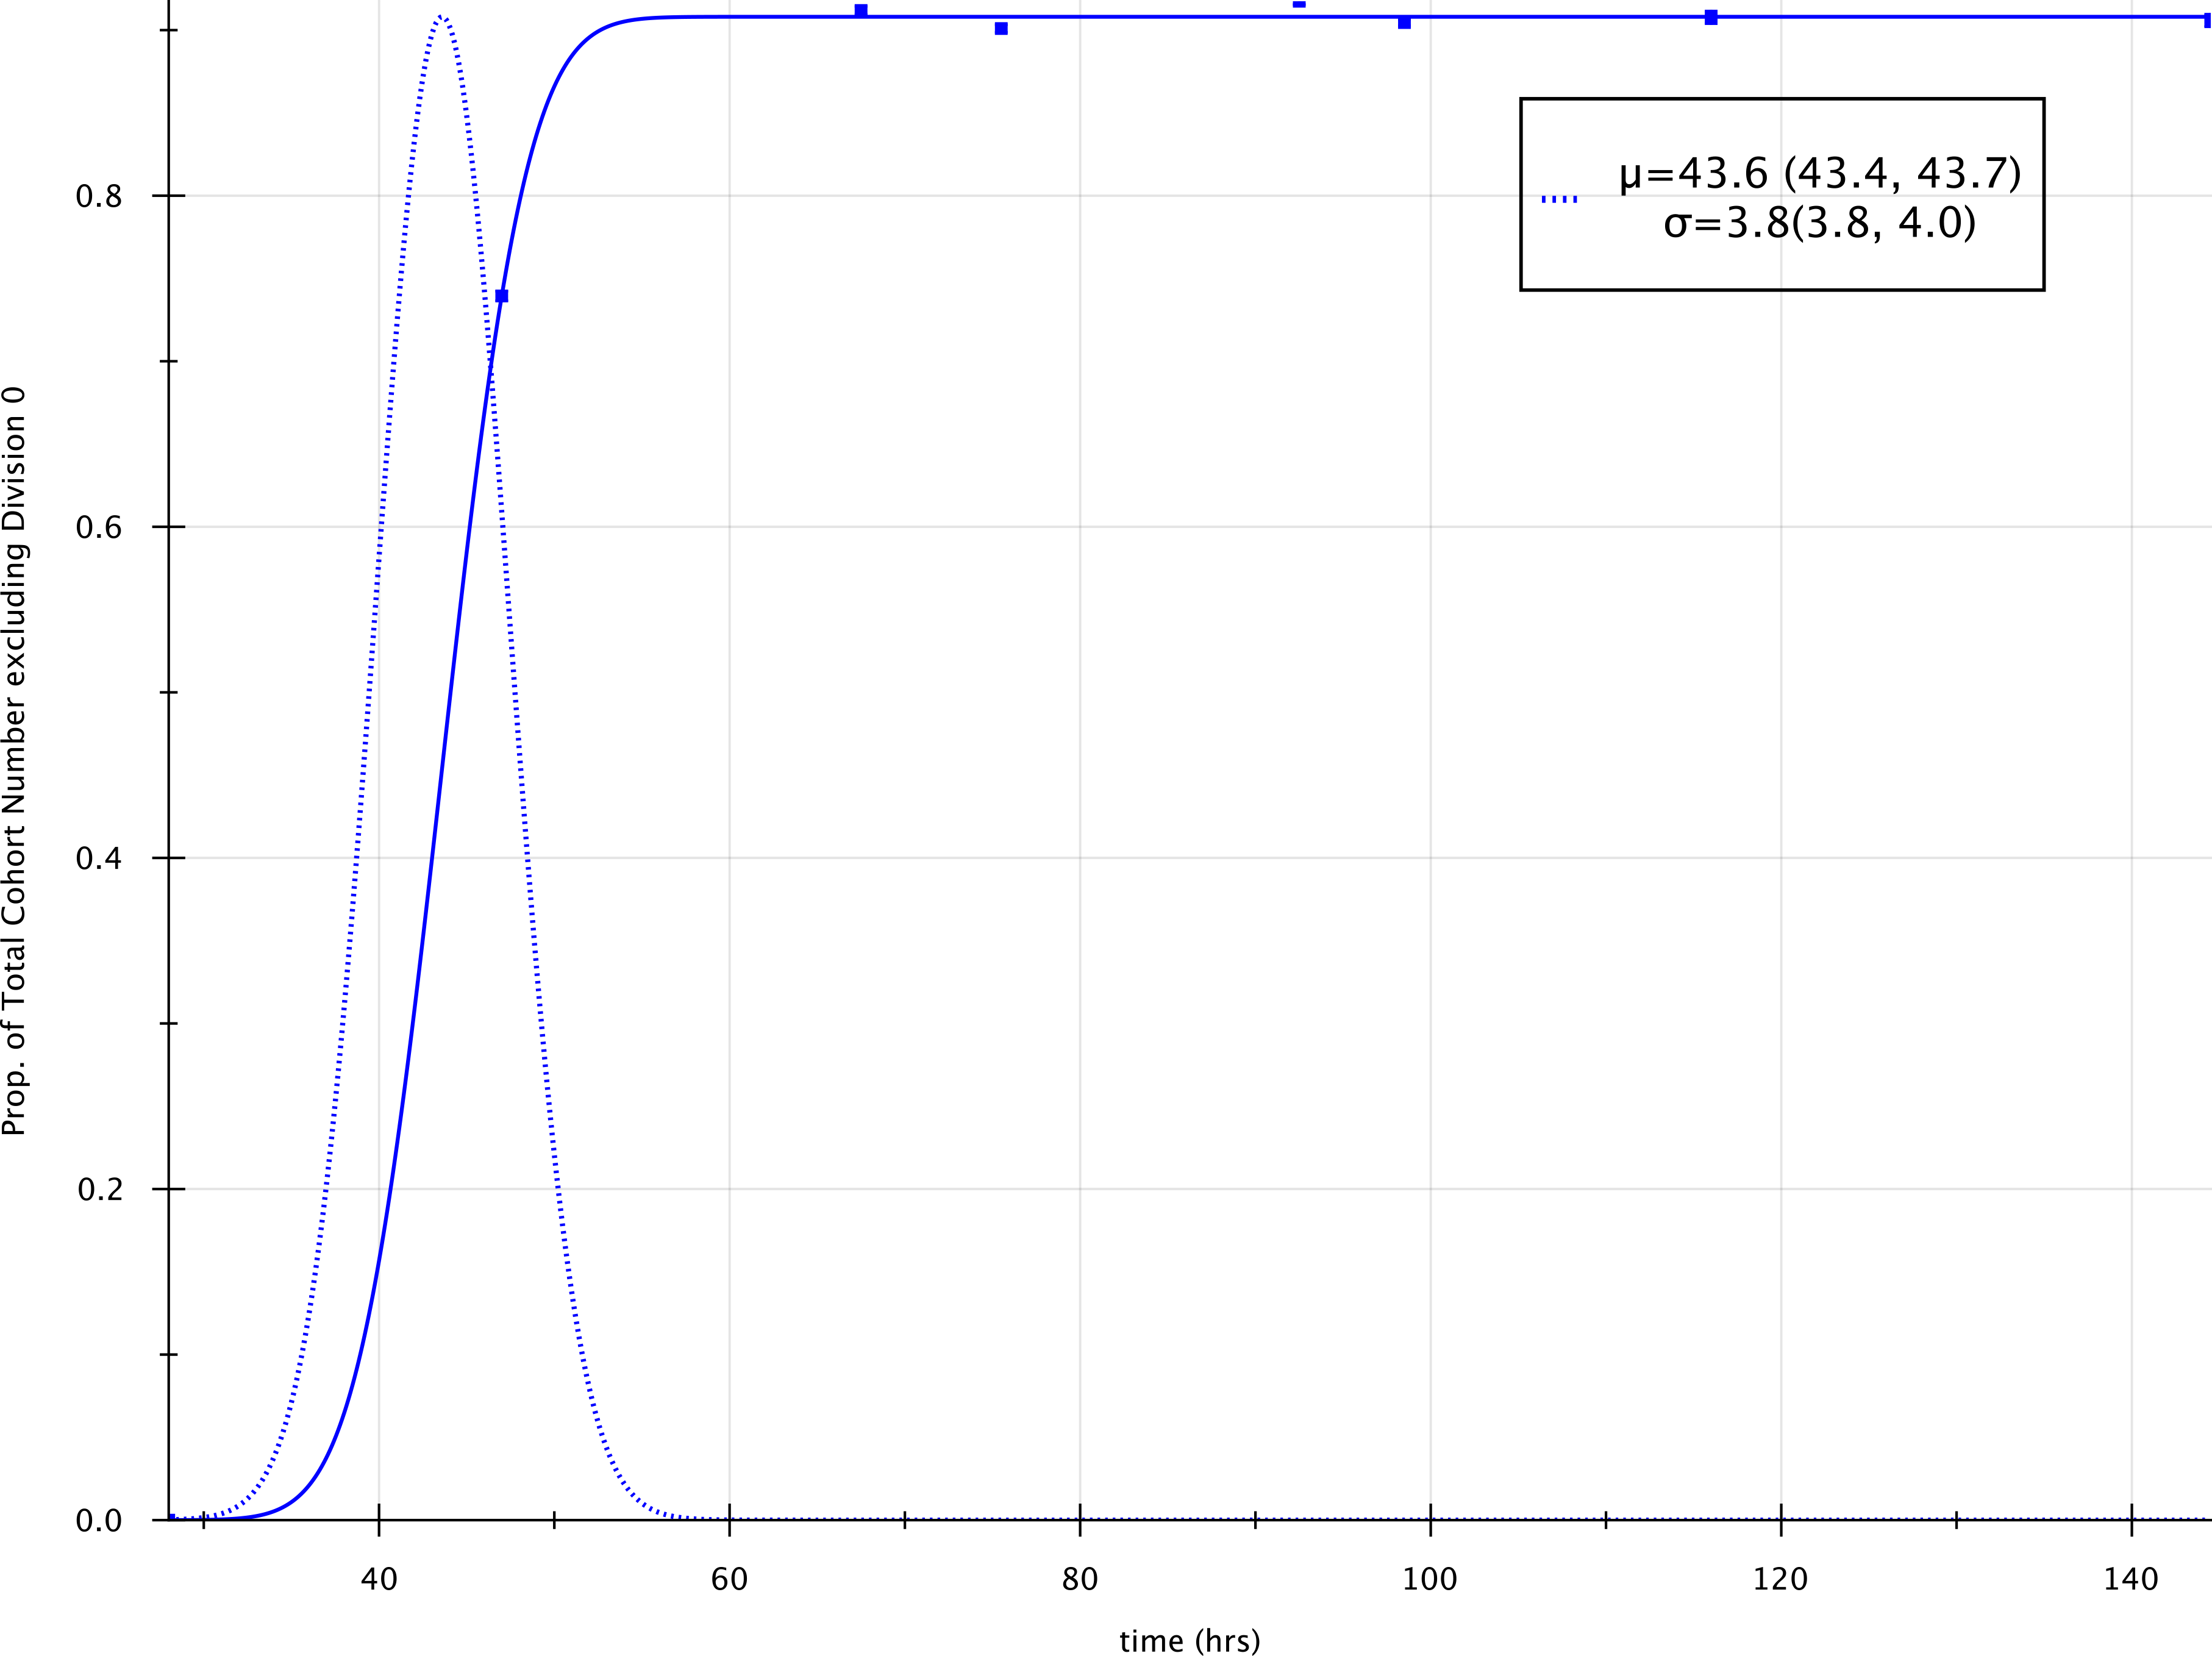
\includegraphics[scale=0.38]{./img/cdf.png}
    \caption{\textbf{An estimated distribution of time to enter first division.} Solid line is best-fit curve to CDF. Dotted line is complementary (continuous) Gaussian distribution. Bootstrap method is utilised to acquire 95\% confidence intervals on each estimated parameters.}
\end{figure}
This is only case where we fit arithmetically computed quantities to estimate a distribution of time to enter first division. Basic idea is that we examine change in ratio of total cohort number excluding division 0 to equation (\ref{eq:total_cohort}). As cells start to divide and enters first division, the ratio approaches a certain value as division 0 cells are cumulatively move into subsequent division.
\begin{equation}
    M(t) = \frac{S_{\mathrm{ex0}}(t)}{S(t)} = \frac{\sum_{k=1} c(k,t)}{\sum_{k=0} c(k,t)}
\end{equation}
if we ignore measurement errors that result in differnt total cell counts per time points, theoretically, it is a bounded function $M(t) \in [0, 1]$. We then fit this equation to cumulative distribution function,
\begin{equation}
    \Phi(t;A,\mu,\sigma) = \frac{A}{2} \left[1 + \erf\left(\frac{t-\mu}{\sigma\sqrt{2}}\right) \right]
\end{equation}
It is again an alternative routine that comparable to parameter tFD in equation (\ref{eq:piecewise_params}).

\end{homeworkProblem}

%----------------------------------------------------------------------------------------
%	SECTION 5 : Bootstrap confidence intervals
%---------------------------------------------------------------------------------------
% \begin{homeworkProblem}[Bootstrapping]
% Goodness-of-fit is measured by bootstrapping input datasets, and cutting off at 95\%. The iteration size can be user-defined by modifying "settings.txt" file.

% \begin{center}
%     I don't think I need to discuss about this?
% \end{center}
% \end{homeworkProblem}

\clearpage
\begin{thebibliography}{9}
\bibitem{Croeze}
Croeze A., L. Pittman \& W. Reynolds (2012)
\textit{Solving nonlinear least-squares problems with the Gauss-Newton and Levenberg-Marquardt methods}.
\url{https://www.math.lsu.edu/system/files/MunozGroup1%20-%20Paper.pdf}

\bibitem{Gett}
Gett A.V. \& Hodgkin P.D. (2000)
\textit{A cellular calculus for signal integration by T cells}.
Nature Immunology.

\bibitem{Griva}
Griva I., Nash S.G. \& Sofer A. (2009)
\textit{Linear and nonlinear optimization}.
Philadelphia, Pennsylvania: siam

\bibitem{Guo}
Guo H. (2011)
\textit{A simple algorithm for fitting a Gaussian function [DSP Tips and Tricks]}.
IEEE Signal Processing Magazine - IEEE SIGNAL PROCESS MAG. 28. 134-137. 10.1109/MSP.2011.941846.

\bibitem{Hawkins}
Hawkins E.D. et al. (2013)
\textit{Quantal and graded stimulation of B lymphocytes as alternative strategies for regulating adaptive immune responses}.
Nature Communications.

\bibitem{Madsen}
Madsen K., Nielsen H.B. \& Tingleff O. (2004)
\textit{Methods for non-linear least squares problems}.
IMM Lecture Note retrieved from \url{http://www2.imm.dtu.dk/pubdb/views/edoc_download.php/3215/pdf/imm3215.pdf}

\bibitem{Marchingo}
Marchingo J.M. et al. (2014)
\textit{Antigen affinity, costimulation, and cytokine inputs sum linearly to amplify T cell expansion}.
Science.

\bibitem{Marsh}
Marsh L., Maudgel M. \& Raman J. (1990)
\textit{Alternative methods of estimating piecewise linear and higher order regression models using SAS software}.
Proceedings of SAS Users Group International 15: 523–527.

\bibitem{Pastuchova}
Pastuchova E. \& Zakopcan M. (2015)
\textit{Comparison of Algorithms For Fitting a Gaussian Function Used in Testing Smart Sensors}.
Journal of Electrical Engineering. 66. 178-181. 10.2478/jee-2015-0029.


\end{thebibliography}


\end{document}
